% This is a template for Ph.D. dissertations in the UCI format.
%
% All fonts, including those for sub- and superscripts, must be 10
% points or larger.  Recommended sizes are 14-point for chapter
% headings, 12-point for the main body of text and figure/table
% titles, and 10-point for footnotes, sub- and super-scripts, and text
% in figures and tables.
%
% Notes: Add short title to figures, sections, via square brackets,
% e.g. \section[short]{long}.
%
\documentclass[12pt,fleqn]{ucithesis}

% A few common packages
\usepackage{amsmath}
\usepackage{amsthm}
\usepackage{array}
\usepackage{graphicx}
\usepackage{natbib}
\usepackage{relsize}

% Some other useful packages
\usepackage{caption}
\usepackage{multirow}
\usepackage{booktabs}
\usepackage{subfigure}

% plainpages=false fixes the "duplicate ignored" error with page counters
% Set pdfborder to 0 0 0 to disable colored borders around PDF hyperlinks
\usepackage[plainpages=false,pdfborder={0 0 0}]{hyperref}

% Uncomment the following two lines to use the algorithm package,
% which provides an algorithm environment similar to figure and table
% ("\begin{algorithm}...\end{algorithm}"). A list of algorithms will
% automatically be added in the preliminary pages. Note that you
% probably want a package for the actual code to go with this (e.g.,
% algorithmic).
%\usepackage{algorithm}
%\renewcommand{\listalgorithmname}{\protect\centering\protect\Large LIST OF ALGORITHMS}

% Uncomment the following line to enable Unicode support. This will allow you
% to enter non-ASCII characters (such as accented characters) directly without
% having to use LaTeX's awkward escape syntax (e.g., \'{e})
% NOTE: You may have to install the ucs.sty package for this to work. See:
% http://www.unruh.de/DniQ/latex/unicode/
%\usepackage[utf8x]{inputenc}

% Uncomment the following to avoid "widowing", where page breaks cause
% single lines of paragraphs to float onto the next page (this is not
% a UCI requirement but more of an aesthetic choice).
%\widowpenalty=10000
%\clubpenalty=10000

% Modify or extend these at will.
\newtheorem{theorem}{\textsc{Theorem}}[chapter]
\newtheorem{definition}{\textsc{Definition}}[chapter]
\newtheorem{example}{\textsc{Example}}[chapter]

% Global variables
\newcommand{\peelingSpeedup}{3.58}

% Macros for title, author, abstract, etc.
\thesistitle{Efficient Hosted Interpreter for Dynamic Languages}

\degreename{Doctor of Philosophy}

% Use the wording given in the official list of degrees awarded by UCI:
% http://www.rgs.uci.edu/grad/academic/degrees_offered.htm
\degreefield{Computer Engineering}

% Your name as it appears on official UCI records.
\authorname{Wei Zhang}

% Use the full name of each committee member.
\committeechair{Professor Michael Franz}
\othercommitteemembers
{
  Professor Kwei-Jay Lin\\
  Professor Guoqing Xu
}

\degreeyear{2015}

\copyrightdeclaration
{
  Portion of Chapter~\ref{chp:ch3-bytecode} {\copyright} $2013$, $2014$ ACM \\
  Portion of Chapter~\ref{chp:ch4-zippy} {\copyright} $2014$ ACM \\
  Portion of Chapter~\ref{chp:ch5-peeling} {\copyright} $2014$ ACM \\
  All other materials {\copyright} {\Degreeyear} \Authorname
}

% If you have previously published parts of your manuscript, you must list the
% copyright holders; see Section 3.2 of the UCI Thesis and Dissertation Manual.
% Otherwise, this section may be omitted.
% \prepublishedcopyrightdeclaration
% {
% 	Chapter 4 {\copyright} 2003 Springer-Verlag \\
% 	Portion of Chapter 5 {\copyright} 1999 John Wiley \& Sons, Inc. \\
% 	All other materials {\copyright} {\Degreeyear} \Authorname
% }

% The dedication page is optional.
\dedications
{

  To my supporting parents and lovely wife.
}

\acknowledgments
{
  First and foremost, I would like to thank my advisor Professor Michael Franz for his mentorship and support during my years in graduate school.
  I am deeply grateful that he admitted me to his fantastic research group and brought me into the world of programming languages.
  Working under his supervision has been one of my most fulfilling period of my life.

  I would also like to thank Professor Kwei-Jay Lin and Professor Guoqing Xu for accepting to serve on my committee.

  I am deeply grateful for Dr. Stefan Brunthaler and Dr. Per Larsen for closely working with me on this research.
  Their continuous guidance, motivation and insightful comments greatly improve me as a graduate student researcher.
  This thesis would not be possible without their help.

  I would also like to thank Dr. Christian Wimmer for his valuable feedback to my work and mentorship during my internships at Oracle Labs.
  I am also grateful to Chris Seaton, Andreas Woess and other people I have worked with at Oracle Labs.
  Their mastery on software design deeply inspired me.

  Lastly, I would like to thank my amazing colleagues.
  I have been fortunate to be a part of this great research group.
  My thanks go to: Mason Chang, Todd Jackson, Michael Bebenita, Christoph Kerschbaumer, Gregor Wagner, Eric Hennigan, 
  Andrei Homescu, G{\"u}lfem Savrun-Yeniçeri, Stephen Crane, Mark Murphy, Codru\c{t} Stancu, Mohaned Qunaibit, Brian Belleville and Julian Lettner.
}


% Some custom commands for your list of publications and software.
\newcommand{\mypubentry}[3]{
  \begin{tabular*}{1\textwidth}{@{\extracolsep{\fill}}p{4.5in}r}
    \textbf{#1} & \textbf{#2} \\
    \multicolumn{2}{@{\extracolsep{\fill}}p{.95\textwidth}}{#3}\vspace{6pt} \\
  \end{tabular*}
}
\newcommand{\mysoftentry}[3]{
  \begin{tabular*}{1\textwidth}{@{\extracolsep{\fill}}lr}
    \textbf{#1} & \url{#2} \\
    \multicolumn{2}{@{\extracolsep{\fill}}p{.95\textwidth}}
    {\emph{#3}}\vspace{-6pt} \\
  \end{tabular*}
}

% Include, at minimum, a listing of your degrees and educational
% achievements with dates and the school where the degrees were
% earned. This should include the degree currently being
% attained. Other than that it's mostly up to you what to include here
% and how to format it, below is just an example.
\curriculumvitae
{

\textbf{EDUCATION}

  \begin{tabular*}{1\textwidth}{@{\extracolsep{\fill}}lr}
    \textbf{Doctor of Philosophy in Computer Engineering} & \textbf{2015} \\
    \vspace{6pt}
    University of California, Irvine & \emph{Irvine, California} \\

    \textbf{Master of Science in Computer Engineering} & \textbf{2010} \\
    \vspace{6pt}
    Chalmers University of Technology & \emph{Gothenburg, Sweden} \\

    \textbf{Bachelor of Science in Mechanical Engineering} & \textbf{2004} \\
    \vspace{6pt}
    University of Science and Technology Beijing & \emph{Beijing, China} \\
  \end{tabular*}

\vspace{12pt}
\textbf{RESEARCH EXPERIENCE}

  \begin{tabular*}{1\textwidth}{@{\extracolsep{\fill}}lr}
    \textbf{Graduate Student Researcher} & \textbf{2010--2015} \\
    \vspace{6pt}
    University of California, Irvine & \emph{Irvine, California} \\

    \textbf{Master Student Researcher} & \textbf{2010} \\
    \vspace{6pt}
    Chalmers University of Technology & \emph{Gothenburg, Sweden} \\
  \end{tabular*}

\vspace{12pt}
\textbf{PROFESSIONAL EXPERIENCE}

  \begin{tabular*}{1\textwidth}{@{\extracolsep{\fill}}lr}
    \textbf{Software Development Intern} & \textbf{Summer 2014} \\
    \vspace{6pt}
    Oracle Labs & \emph{Belmont, CA} \\

    \textbf{Software Development Intern} & \textbf{Summer 2013} \\
    \vspace{6pt}
    Oracle Labs & \emph{Belmont, CA} \\

    \textbf{Customer Service Engineer} & \textbf{2007--2008} \\
    \vspace{6pt}
    ASML & \emph{Shanghai, China} \\

    \textbf{Production Engineer} & \textbf{2005--2007} \\
    \vspace{6pt}
    AT\&S & \emph{Shanghai, China} \\

    \textbf{Mechanical Design Engineer} & \textbf{2004--2005} \\
    \vspace{6pt}
    BMEI & \emph{Beijing, China} \\
  \end{tabular*}

\pagebreak

\textbf{PUBLICATIONS}

  % \mypubentry{Awesome paper}{Jun 2011}{Conference name}
  % \mypubentry{Another awesome paper}{Aug 2012}{Conference name}

Wei Zhang, Per Larsen, Stefan Brunthaler, Michael Franz.
\textbf{Accelerating Iterators in Optimizing AST Interpreters}.
\textit{In Proceedings of the 29th ACM SIGPLAN Conference on Object Oriented Programming:
Systems, Languages, and Applications, Portland, OR, USA, October 20-24, 2014 (OOPSLA '14)}, 2014.

G{\"u}lfem Savrun-Yeniçeri, Wei Zhang, Huahan Zhang, Eric Seckler, Chen Li, Stefan Brunthaler,
Per Larsen, Michael Franz.
\textbf{Efficient Hosted Interpreters on the JVM}.
\textit{In ACM Transactions on Architecture and Code Optimization, volume 11(1) pages 9:1–9:24}, 2014.

G{\"u}lfem Savrun-Yeniçeri, Wei Zhang, Huahan Zhang, Chen Li, Stefan Brunthaler, Per Larsen, Michael Franz.
\textbf{Efficient Interpreter Optimizations for the JVM}.
\textit{In Proceedings of the 10th International Conference on Principles and Practice of Programming in Java,
Stuttgart, Germany, September 11-13, 2013 (PPPJ '13)}, 2013.

\vspace{12pt}
\textbf{SOFTWARE}

\mysoftentry{ZipPy}{http://bitbucket.org/ssllab/zippy/}
{A fast and lightweight Python 3 implementation built using the Truffle framework.
It leverages the underlying Java JIT compiler and compiles Python programs to highly optimized machine code at runtime.}

\mysoftentry{ModularVM}{https://bitbucket.org/thezhangwei/modularvm/}
{An extension to the Maxine VM (Java Virtual Machine) that enables deeper integrations with JVM languages
like Jython (Python), Rhino (JavaScript) or JRuby (Ruby). It automatically accelerates guest language interpreters written in Java.}

}

% The abstract should not be over 350 words, although that's
% supposedly somewhat of a soft constraint.
\thesisabstract
{

Motivated by high development costs, production compilers and virtual machines, often support more than one language.
This strategy is most effective when the language family is homogeneous.
Many languages are very amenable to static program analysis, however, dynamic languages are not.
Consequently, a single VM cannot deliver peak performance for both types of languages without adapting its optimization strategy accordingly.

Informally, we host a ``highly dynamic'' language (Python) on the Java Virtual Machine, a VM for ``moderately dynamic'' languages.
While we are not the first to do so, our approach diverges from current practice by representing Python programs as abstract syntax trees, ASTs, rather than bytecode.
Not only are ASTs the simplest and most natural programming language implementation,
they also lend themselves well to optimizations those are particularly beneficial to highly dynamic languages.
Compared to Jython, which compiles Python programs to Java bytecode, our Python prototype is faster and requires less implementation effort.

}


%%% Local Variables: ***
%%% mode: latex ***
%%% TeX-master: "thesis.tex" ***
%%% End: ***


% Add PDF document info fields
\hypersetup{
	pdftitle={\Thesistitle},
	pdfauthor={\Authorname},
	pdfsubject={\Degreefield},
}

% Uncomment the following to have numbered subsubsections (by default
% numbering goes only to subsections).
%\setcounter{secnumdepth}{4}


% Set this to only select a subset of the includes directives below.
% Very handy to speed up compilation if you're working on a certain
% part of your thesis. It conserves page numbers, references, etc.
% even for non-included files.
%\includeonly{chapter1}

\begin{document}

% Preliminary pages are always loaded (TOC, CV, etc.)
\preliminarypages

% Include the different components of your thesis, in separate files.
% Using \include allows you to set \includeonly above.
\chapter{Introduction}

This is an example using the \LaTeX{} template for UCI theses and
dissertation documents \cite{uci-thesis-latex}. Figure
\ref{fig:sourcecode} is just for illustration purposes, as is Table
\ref{tab:coordinates}.

\begin{figure}
\begin{verbatim}
#include <iostream>
int main(int argc, char** argv) {
  std::cout << "Hello World." << std::endl;
  return 0;
}
\end{verbatim}
  \caption{Example source code.}
  \label{fig:sourcecode}
\end{figure}

\section{Background}

Lorem ipsum dolor sit amet, consectetur adipisicing elit, sed do
eiusmod tempor incididunt ut labore et dolore magna aliqua. Ut enim ad
minim veniam, quis nostrud exercitation ullamco laboris nisi ut
aliquip ex ea commodo consequat. Duis aute irure dolor in
reprehenderit in voluptate velit esse cillum dolore eu fugiat nulla
pariatur. Excepteur sint occaecat cupidatat non proident, sunt in
culpa qui officia deserunt mollit anim id est laborum.

\begin{table}
  \centering
  \begin{tabular}{|rr|r|}
    \hline
    $x$ & $y$ & $z$ \\
    \hline
    14 & 12 & -2 \\
    0 & 33 & -25 \\
    -3 & 11 & 22 \\
    4 & 4 & 6 \\
    \hline
  \end{tabular}
  \caption{Example coordinates.}
  \label{tab:coordinates}
\end{table}

Lorem ipsum dolor sit amet, consectetur adipisicing elit, sed do
eiusmod tempor incididunt ut labore et dolore magna aliqua. Ut enim ad
minim veniam, quis nostrud exercitation ullamco laboris nisi ut
aliquip ex ea commodo consequat. Duis aute irure dolor in
reprehenderit in voluptate velit esse cillum dolore eu fugiat nulla
pariatur. Excepteur sint occaecat cupidatat non proident, sunt in
culpa qui officia deserunt mollit anim id est laborum.


%%% Local Variables: ***
%%% mode: latex ***
%%% TeX-master: "thesis.tex" ***
%%% End: ***

\chapter{Hosted Bytecode Interpreter}

A programming language interpreter executes programs in two steps.
First it parses the human readable source code, verifies its correctness and translates the code into a more efficient intermediate representation (IR) format.
The interpreter then picks up the translated program and executes it piece by piece.

Bytecode interpreters parse source program into bytecode, a highly compressed representation of the program.
The format of the bytecode is a form of virtual instruction set designed for this particular interpreter.
In the second step bytecode interpreters execute the bytecode as a sequence of virtual instruction one instruction at a time before finishing the last one.
Interpreters are also regard as virtual machines, since they emulate ``machines'' with their own virtual instruction sets.

In this Chapter, we go over performance overheads of bytecode interpreters and the classic techniques used to minimize these overheads.
Lastly, we introduce ModularVM~\cite{savrun2013, savrun2014}, a research JVM that automatically optimize the performance of hosted bytecode interpreters.

\section{Performance Anatomy of Bytecode Interpreters}

Bytecode interpreters execute bytecode one instruction at a time.
For each instruction, the interpretation consists of three steps~\cite{davis2003case}:
\begin{itemize}
  \item Instruction dispatch
  \item Operand access
  \item Performing the function of the instruction
\end{itemize}
Instruction dispatch includes fetching the next instruction, decoding the instruction and transferring program execution to the actual implementation of the instruction.
Operand access involves fetching operands required to perform the instruction from either a temporal operand stack or a virtual register file depending on the design of the virtual instruction set.
It also includes storing the computed result back to where temporal operands should be stored.
Subsequently in the last step the interpreter performs the actual computation.
For instance, if the instruction is addition of two numbers, the actually addition is performed in this step.

\begin{figure}[th]
\centering
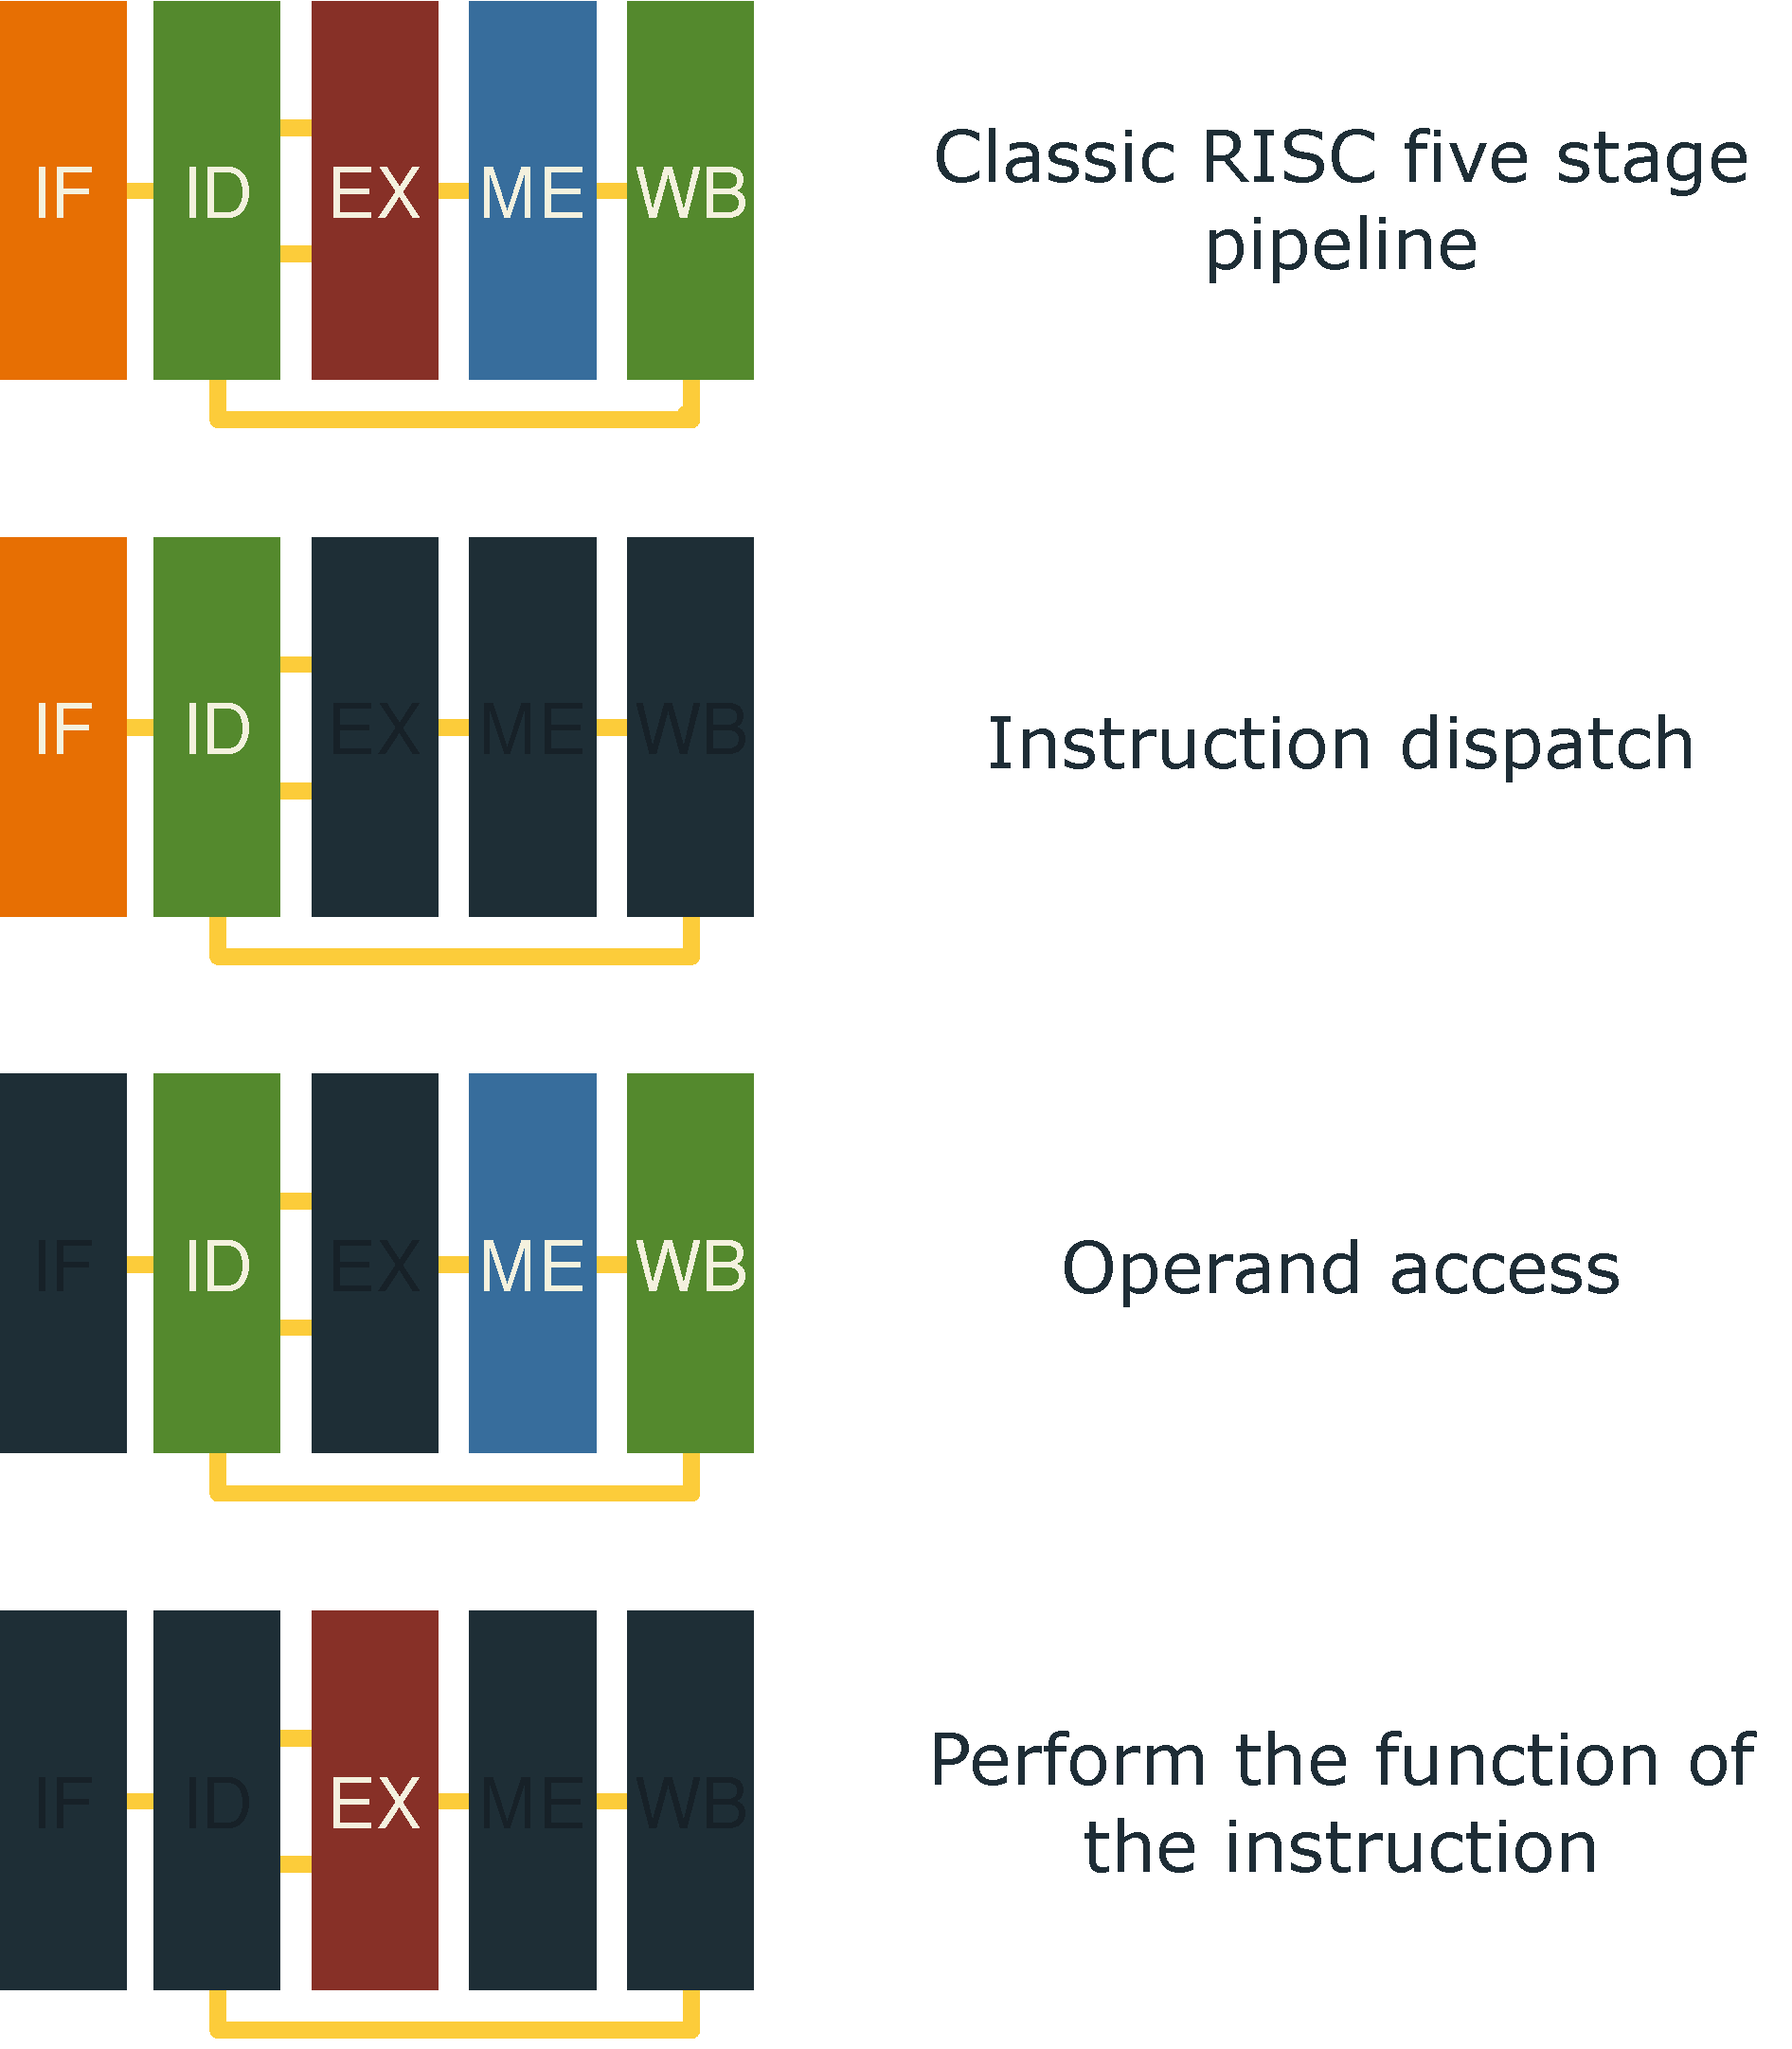
\includegraphics[scale=.25]{figures/ch2-risc-pipeline.pdf}
\caption{Interpretation costs of bytecode interpreters}
\label{fig:interpretation-cost}
\end{figure}

An interesting way to further illustrate the purpose of each interpretation step
from the angle of a virtual machine is to correlate them with the stages in a classic reduced instruction set computer (RISC) pipeline.
Figure~\ref{fig:interpretation-cost} illustrates the five stages in a classic RISC pipeline:
instruction fetch (IF), instruction decode (ID), execute (EX), memory access (ME) and write back (WB).
The instruction dispatch step in bytecode interpreters is similar to instruction fetch and decode stages in RISC.
We can correlate the late stage of instruction decode, memory access and write back in RISC to operand access in an interpreter.
Since these are the stages that prepare the operands for the computing unit and stores the end result back to either a register or memory address.
The interpreter step that performs the function of the instruction works exactly as the execute stage in RISC, which performs the actual computation.

The cost of running a hosted program on an interpreter consists of the costs of performing each of the three steps we described above.
Among those steps, instruction dispatch and operand access does not directly contribute to the actual work of the hosted program.
The less time the interpreter spend in these two steps, the more time the interpreter spend in doing the actual work.
Therefore, an efficient bytecode interpreter must encompass techniques that optimize instruction dispatch and operand access.

\subsection{Switch-based Dispatch}

\begin{figure}[th]
\centering
\subfigure[dispatch loop] {
  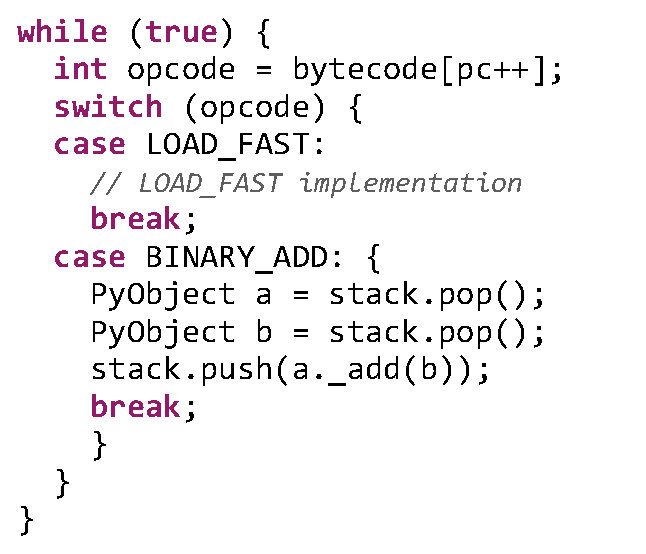
\includegraphics[scale=.70]{figures/ch2-switch-based-dispatch-code.pdf}
  \label{fig:switch-based-dispatch-code}
}
\subfigure[branches in switch-based dispatch] {
  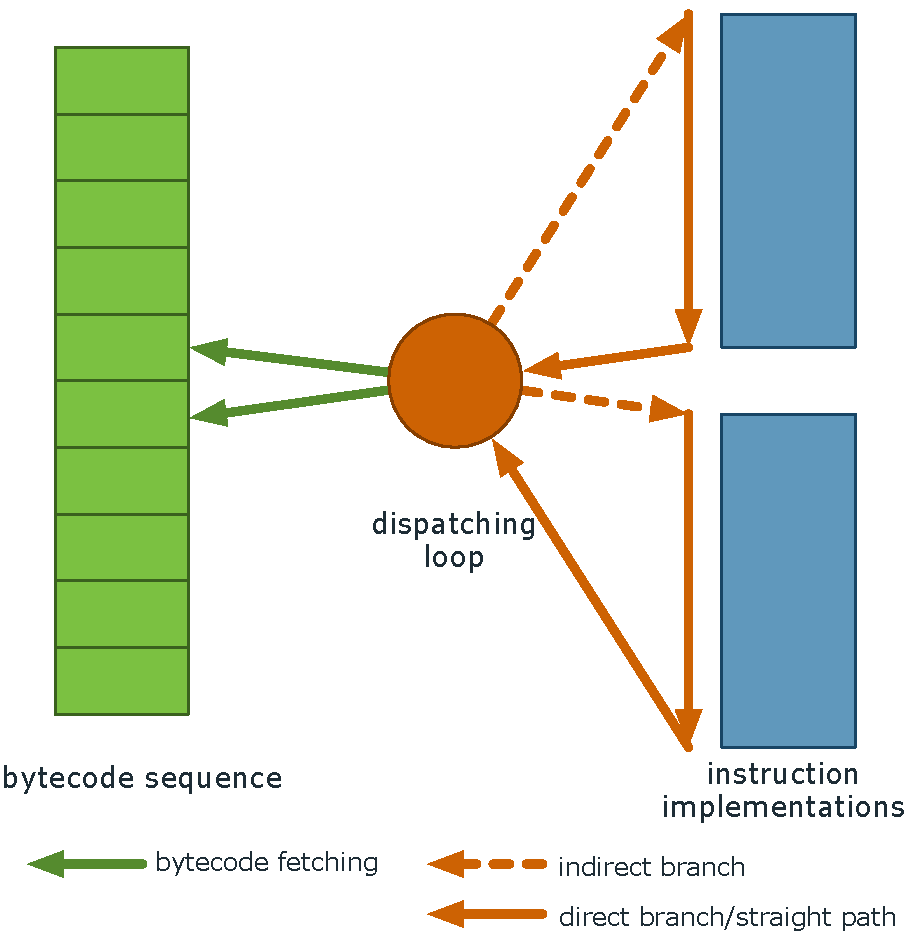
\includegraphics[scale=.47]{figures/ch2-switch-based-dispatch-branch.pdf}
  \label{fig:switch-based-dispatch-branch}
}
\caption{switch-based dispatch}
\label{fig:switch-based-dispatch}
\end{figure}

The simplest way to construct a bytecode interpreter is to use an interpreter loop and a switch statement in the loop to dispatch each bytecode instruction.
Figure~\ref{fig:switch-based-dispatch-code} illustrates a switch-based bytecode interpreter loop written in Java.
In each iteration of the loop, the interpreter fetches the next instruction and use the switch statement to redirect execution to the case block that implements the instruction.
Figure~\ref{fig:switch-based-dispatch-branch} shows the branches involved in a switch-based dispatch.
Note that each iteration of the dispatch loop shares the same indirect branch.
Since the bytecode sequence is input dependent and unlikely to form a predictable pattern,
branch prediction mechanisms in modern hardware tend to mis-predict the shared indirect branch.
This mis-prediction results in a significant performance penalty for switch-based bytecode interpreters.

\section{Efficient Instruction Dispatch Techniques}
\label{sec:efficient-instruction-dispatch-techniques}

\subsection{Direct Threading Dispatch}
\label{sec:direct-threading-dispatch}

\begin{figure}[th]
\centering
\subfigure[direct threading interpreter] {
  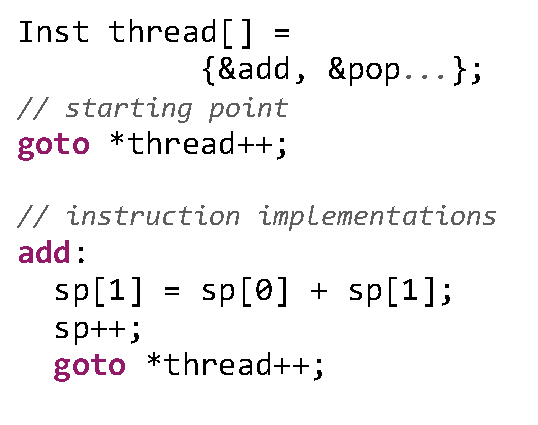
\includegraphics[scale=.85]{figures/ch2-direct-threading-dispatch-code.pdf}
  \label{fig:direct-threading-dispatch-code}
}
\subfigure[branches in direct threading dispatch] {
  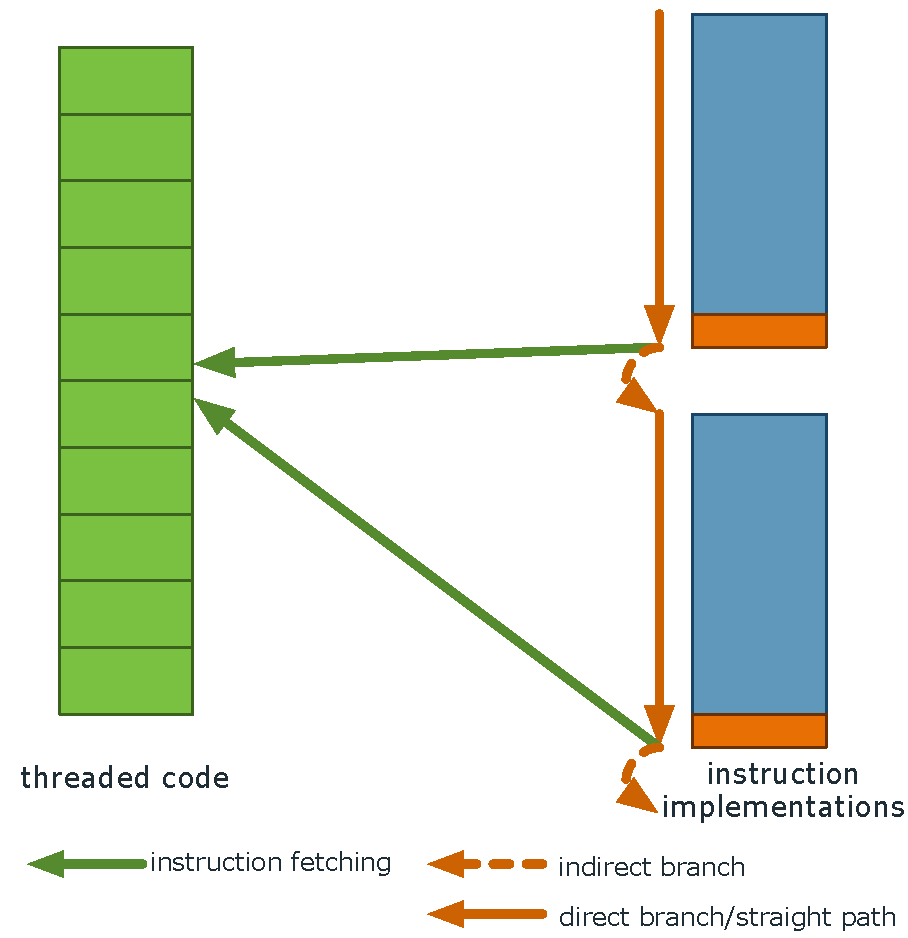
\includegraphics[scale=.47]{figures/ch2-direct-threading-dispatch-branch.pdf}
  \label{fig:direct-threading-dispatch-branch}
}
\caption{direct threading dispatch}
\label{fig:direct-threading-dispatch}
\end{figure}

Instead of letting each instruction dispatch share the same branch, direct threading duplicates instruction dispatch at the end of each instruction implementation~\cite{bell73}.
Figure~\ref{fig:direct-threading-dispatch-code} illustrates this technique written in C.
Direct threading requires an additional translation phase that translates the bytecode sequence into a sequence of pointers or the threaded code.
Each pointer in the threaded code points to the instruction implementation that corresponds to the bytecode instruction in the original bytecode input.
The interpreter starts interpretation by jumping to the address pointed by the first pointer in the threaded code as shown in Figure~\ref{fig:direct-threading-dispatch-code}.
Similarly each instruction implementation repeat the same dispatch routine at the end of it to forward execution to the next instruction implementation.
The duplicated dispatch branches reduce indirect branch mis-predictions.
Therefore, direct threading alleviates the performance loss we have seen in switch-based dispatch.

\subsection{Subroutine Threading Dispatch}

\begin{figure}[th]
\centering
\subfigure[subroutine threaded code] {
  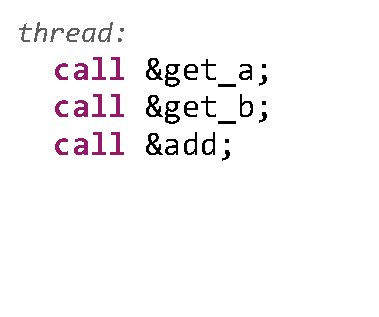
\includegraphics[scale=.85]{figures/ch2-subroutine-threading-dispatch-code.pdf}
  \label{fig:subroutine-threading-dispatch-code}
}
\subfigure[branches in subroutine threading dispatch] {
  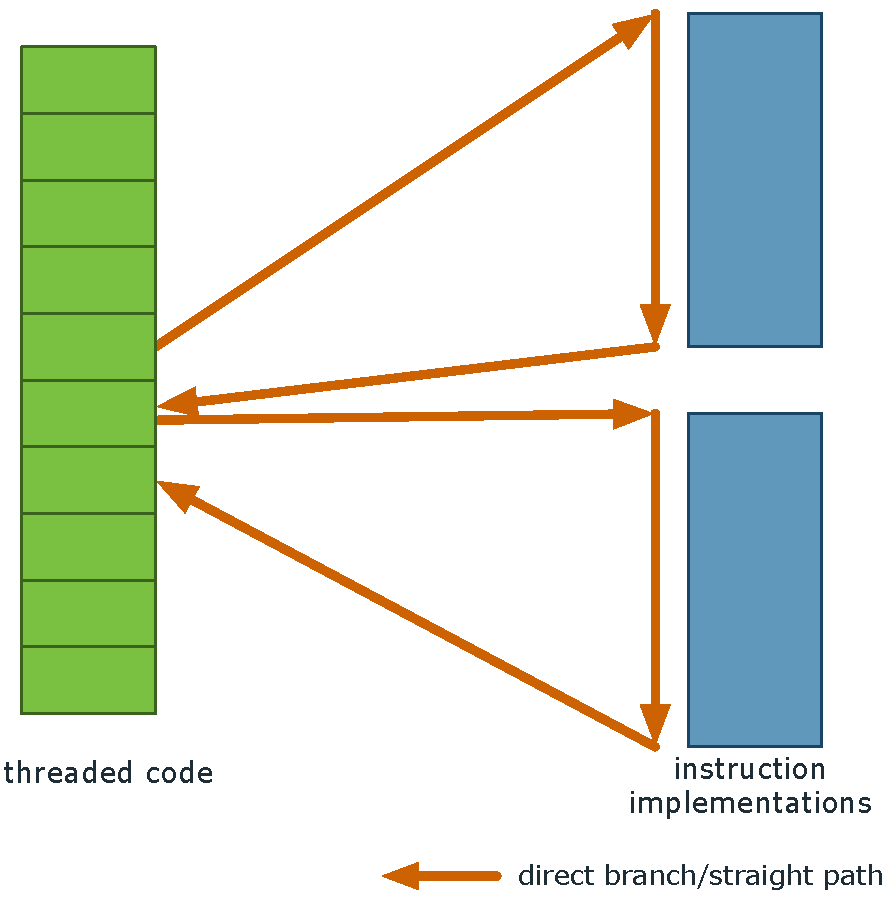
\includegraphics[scale=.47]{figures/ch2-subroutine-threading-dispatch-branch.pdf}
  \label{fig:subroutine-threading-dispatch-branch}
}
\caption{subroutine threading dispatch}
\label{fig:subroutine-threading-dispatch}
\end{figure}

Subroutine threading takes one step further by translating the input bytecode sequence directly to executable machine code.
The translated machine code or the subroutine threaded code is a sequence of machine level calls.
Each call is a direct branch jumping to an instruction implementation as a subroutine.
The subroutine threaded code translation phase translates each input bytecode to a subroutine call to the corresponding instruction implementation.
Each instruction implementation ends with a return instruction that transfer execution back to the threaded code.
Note that the call instruction in subroutine threading is a direct branch.
Although the return instruction is an indirect branch, modern hardware can accurately predict call/return repairs which results in a performance increase.

\section{Efficient Instruction Dispatch for Hosted Bytecode Interpreters}

Instruction dispatch greatly affects the overall performance of a bytecode interpreter.
The implementation of an efficient instruction dispatch technique like the ones explained in Chapter~\ref{sec:efficient-instruction-dispatch-techniques}
relies on the use of computed goto's.
Due to the restricted use of pointers, a hosted bytecode interpreter written in Java can not make use of those techniques.
To address this issue, we extend the JVM by adding the functionality of threaded code generation to enable efficient instruction dispatch for hosted interpreters.
Our research prototype takes an existing switch-based bytecode interpreter written in Java, and converts it into a direct threading interpreter in a semi-automatic fashion.

\subsection{System Overview}

\begin{figure}[th]
\centering
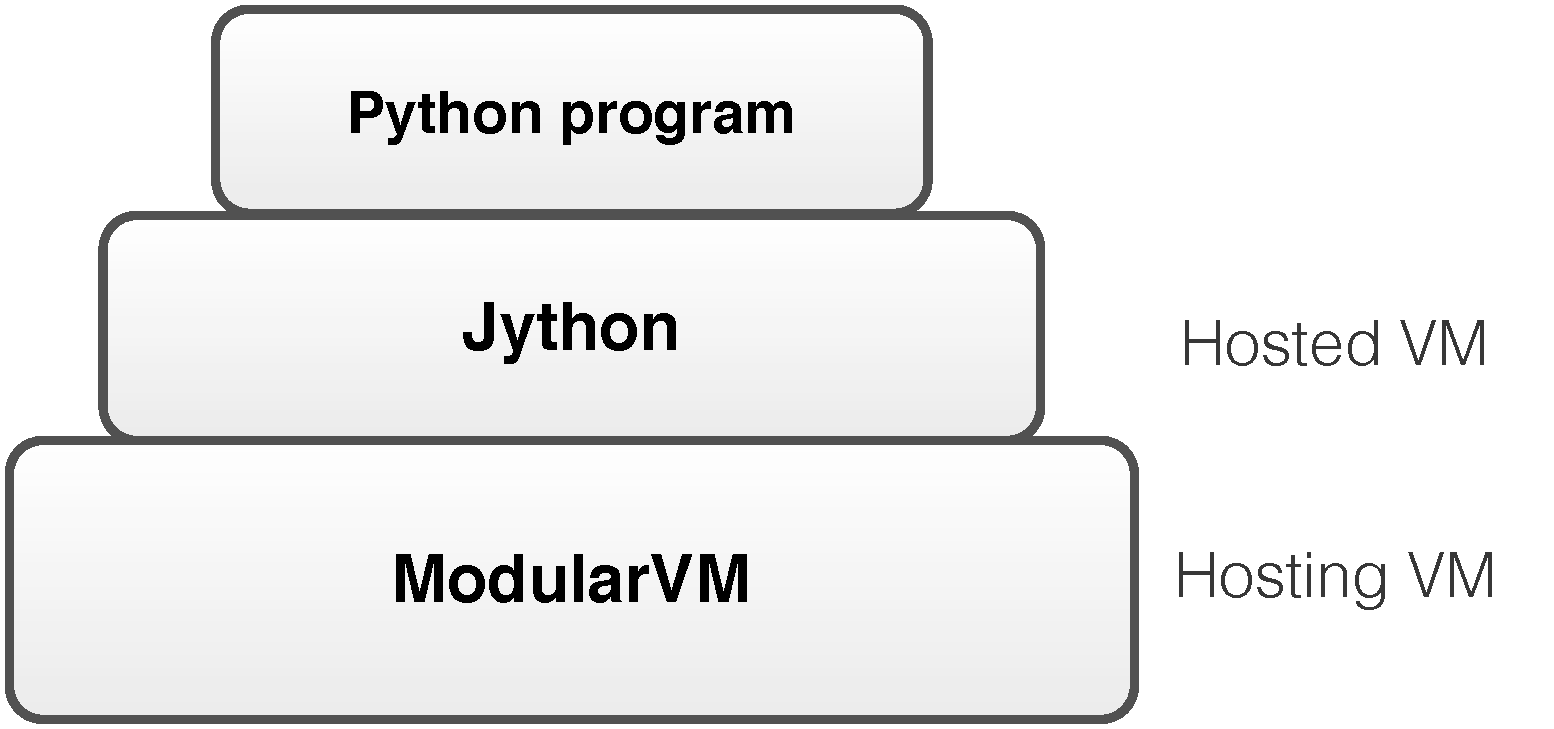
\includegraphics[scale=.3]{figures/ch2-jython-on-modularvm.pdf}
\caption{Jython on ModularVM}
\label{fig:jython-on-modularvm}
\end{figure}

Our system, Modular VM, is an extension to Maxine VM~\cite{Wimmer2013}, a research JVM developed at Oracle Labs.
We build Modular VM with the ability to recognize hosted interpreters running on top of it and automatically optimizes them.
We host Jython, a Python VM written in Java, on Modular VM in our experiment to show case our optimization.
Figure~\ref{fig:jython-on-modularvm} illustrates the overall system setup.
Modular VM hosts Jython like other regular JVMs.
Jython executes Python program in two fashions: using the baseline bytecode interpreter or
compiling Python code to Java bytecode and let the JVM compiler further compile it down to machine code.
Our optimization focuses on the bytecode interpreter.
It shows that by incorporating efficient interpreter optimizations, bytecode interpreter can deliver comparable performance to a basic compiler.

\subsection{Threaded Code Generation}

\begin{figure}[!h]
\centering
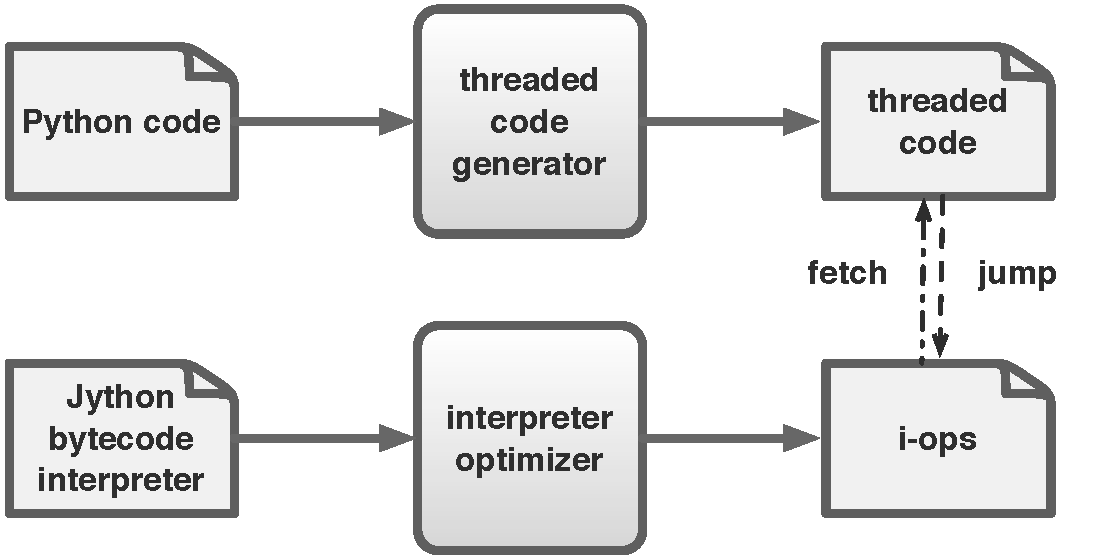
\includegraphics[scale=.5]{figures/ch2-direct-threading-on-modularvm.pdf}
\caption{Threaded code generation}
\label{fig:direct-threading-on-modularvm}
\end{figure}

Modular VM performs threaded code generation in two steps.
First, it recognizes the hosted interpreter running on top of it and transforms it into an optimized one.
To be more specific, Modular VM extracts all the bytecode instruction implementations or i-ops for short from the interpreter and
compiles them into machine code using the existing Java compiler.
Modular VM then initializes an i-op code table that contains the address of all the compiled i-ops.
After this transformation, the interpreter is ready to execute Python programs.
It first translates Python source code to Python bytecode and then further translates bytecode to direct threaded code using the i-op code table.
The generated threaded code is a sequence of code pointers copied from the i-op code table.

Figure~\ref{fig:direct-threading-on-modularvm} illustrates this work flow.
The interpreter optimizer in the Figure applies the transformation to Jython's bytecode interpreter.
Subsequently, the thread code generator produces threaded code and executes it.
Both interpreter optimizer and threaded code generator are part of Modular VM.
Our system encapsulates the details of i-ops compilation and threaded code generation from the hosted VM.

\subsubsection{Interpreter Annotation}

\begin{figure}[ht]
\centering
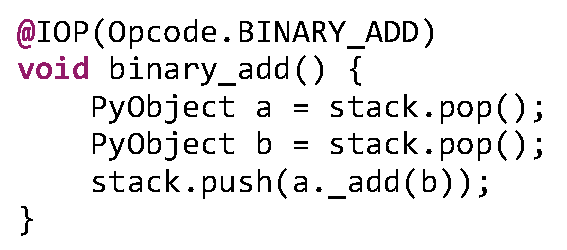
\includegraphics[scale=.65]{figures/ch2-annotated-iop-code.pdf}
\caption{Annotated i-op}
\label{fig:annotated-iop}
\end{figure}

Modular VM uses a Java annotation based domain specific language to integrate with the hosted interpreter.
Our programmable interface provides a set of annotations for hosted VM implementers to annotate different components of their interpreter.
We expect hosted VM implementers to properly annotate the interpreter class, the bytecode class and all the i-op methods for our system to identify the structure of the interpreter.
Figure~\ref{fig:annotated-iop} shows an annotated i-op in Jython's bytecode interpreter refactored to its own separate method.
Modular VM automatically picks up Java methods annotated as i-ops, optimizes them and put them into the i-op code table.

\subsubsection{Next Dispatch}

\begin{figure}[ht]
\centering
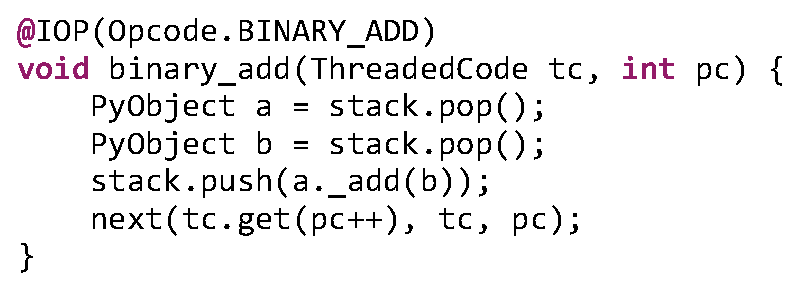
\includegraphics[scale=.65]{figures/ch2-iop-with-next-code.pdf}
\caption{I-op with next dispatch}
\label{fig:iop-with-next}
\end{figure}

Direct threading, as explained in Chapter~\ref{sec:direct-threading-dispatch}, duplicates instruction dispatch at the end of each instruction implementation or i-op.
When the interpreter optimizer compiles an i-op, it also insert a synthesized \emph{next} routine at the end of the i-op.
The \emph{next} routine performs the actual instruction dispatch.
Figure~\ref{fig:iop-with-next} illustrates the i-op of \texttt{BINARY\_ADD} in Jython with the \emph{next} routine.
Note that the figure shows what the program looks like with the added instruction dispatch.
Hosted VM implementers are not required to write the additional code.
As shown in Figure~\ref{fig:iop-with-next}, the intrinsic function \texttt{next} performs an indirect jump to the next i-op in the threaded code.
The \emph{next} routine also passes the reference to the threaded code and virtual program pointer to the next instruction to continue the execution of the program.

\subsubsection{Stack Frame Reusing}

As described above, the \texttt{next} instruction dispatch performs a native indirect branch instead of a call.
Therefore, i-ops need to reuse the same stack frame allocated for each Python function invocation.
We implement this using two special i-ops, \texttt{PROLOGUE} and \texttt{EPILOGUE}.
Both of them are manually assembled instead of compiled from Java source code.
\texttt{PROLOGUE}, used at the beginning of a function, allocates a stack frame that is big enough to accommodate all i-ops.
\texttt{EPILOGUE}, used to model \texttt{RETURN}, deallocates the stack frame and returns.
The interpretation of a Python method always start with a \texttt{PROLOGUE} and end with an \texttt{EPILOGUE}.
Stack frame reusing reduces the number of native machine instructions executed for each hosted virtual machine instruction dispatch.

\subsubsection{Efficient Array Stores}
\label{sec:efficient-array-stores}

Another problem affecting hosted interpreter performance on the JVM is the performance of array stores.
Java being a safe language performs type check such as \texttt{ArrayStoreException} checks on array stores.
Hosted language interpreters like the one in Jython uses an operand stack to manage temporal operands.
Internally, the operand stack is implemented as an Java object array.
During interpretation, every i-op that produces a value performs an array store onto the operand stack.
As a result, the interpreter repeatedly performs the same the type check, even though every i-op is guaranteed to produce an value that is safe to be stored on the operand stack.

We identified the detrimental effect of preserving array type-safety for hosted interpreters.
Our interpreter optimizer omits the \texttt{ArrayStoreException} checks when compiling the i-ops of hosted interpreters.

\subsubsection{An Example}

\begin{figure}[th]
\centering
\subfigure[Python source code] {
  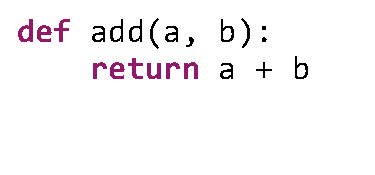
\includegraphics[scale=.85]{figures/ch2-threaded-code-example-python.pdf}
  \label{fig:threaded-code-example-python}
}
\subfigure[Python bytecode] {
  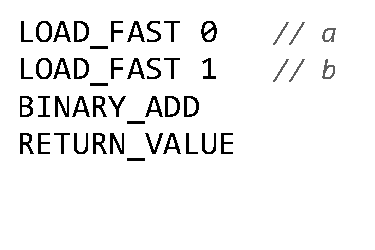
\includegraphics[scale=.75]{figures/ch2-threaded-code-example-bytecode.pdf}
  \label{fig:threaded-code-example-bytecode}
}
\subfigure[Threaded code] {
  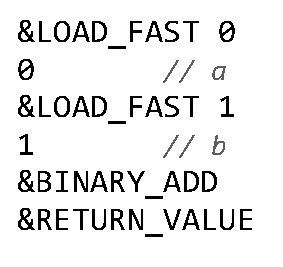
\includegraphics[scale=.7]{figures/ch2-threaded-code-example-threaded-code.pdf}
  \label{fig:threaded-code-example-threaded-code}
}
\caption{Direct threading example}
\label{fig:threaded-code-example}
\end{figure}

Figure~\ref{fig:threaded-code-example} illustrates the Python program translation in Jython hosted on Modular VM.
The input program, as shown in Figure~\ref{fig:threaded-code-example-python}, is a simple Python method that adds two parameters.
Jython first converts the program to the bytecode sequence show in Figure~\ref{fig:threaded-code-example-bytecode}.
Note that the bytecode instruction \texttt{LOAD\_FAST} consists of not only the \texttt{LOAD\_FAST} opcode itself but also an opcode argument ($0$ or $1$) in the bytecode sequence.
Figure~\ref{fig:threaded-code-example-threaded-code} shows the direct threading code produced by the threaded code generator.
Aside from the translated i-op addresses, the threaded code generator also copies opcode arguments, like the one in \texttt{LOAD\_FAST}, into the threaded code.

\section{Evaluation}

\chapter{Hosted AST Interpreter}

Abstract syntax trees, ASTs, are the simplest and most natural ways to implement programming languages.
They do not require an additional translation step that linearizes ASTs produced by the parser to bytecode or other forms of internal representations.
They also lend themselves well to optimizations that are particularly beneficial to highly dynamic languages like Python.

We present ZipPy, a Python 3 implementation that is hosted on the JVM.
ZipPy incorporates recent works on self-optimizing AST interpreters for the JVM.
Our work however focuses on high level guest language features that are distinct in Python and
how well we can fit them onto the existing optimizing AST interpreter framework.

\section{Python on Truffle}

\begin{figure}[t]
\centering
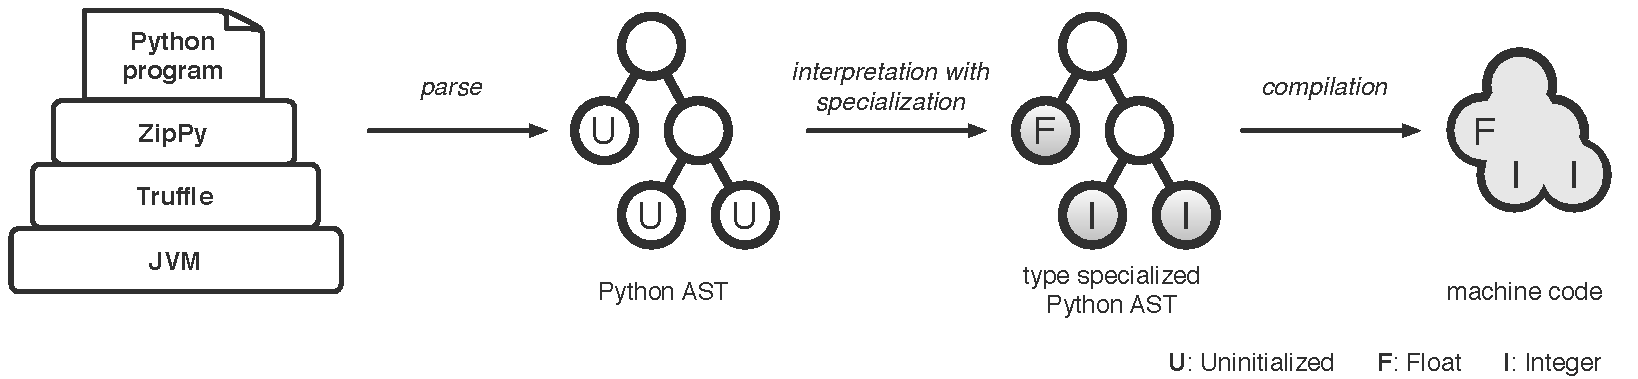
\includegraphics[scale=.6]{figures/ch3-python-on-truffle.pdf}
\caption{Python on Truffle}
\label{fig:python-on-truffle}
\end{figure}

In principle, ``everything'' can change at any moment in dynamic language programs.
This dynamic nature is the major impediment to ahead-of-time optimization.
In practice, however, programmers tend to minimize the rate of change, which makes the code highly predictable.
Types, for instance, typically remain stable between successive executions of a particular operation instance.
Deutsch and Schiffman report that speculative type specialization succeeds $95\%$ of the time in their classic Smalltalk-80 implementation~\cite{Deutsch1984}.

Truffle is a self-optimizing runtime system that makes it easy to perform type specialization for dynamic languages running on top of the JVM~\cite{Wurthinger+13}.
It allows language implementers to implement their guest language by writing an AST interpreter using Java.
An interpreter written in this way enjoys low cost type specialization via automatic node rewriting~\cite{Wurthinger+12,Brunthaler2010inca,Brunthaler2010quickening}.
AST node rewriting collects runtime type information, and speculatively replaces the existing nodes with specialized and more efficient ones.
Subsequently, Truffle just-in-time compiles the specialized AST, written in Java, directly to machine code using the underlying Java compiler.
Upon a type mis-speculation, the specialized AST node handles the type change by replacing itself with a more generic one.
The node replacement triggers deoptimization from the compiled code and transfers execution back to the interpreter.
If the re-specialized AST stays stable, Truffle can again compile it to machine code.

Our system, ZipPy, is a full-fledged prototype Python 3 implementation built atop Truffle.
It leverages Truffle's type specialization feature and its underlying compilation infrastructure (see Figure~\ref{fig:python-on-truffle}).
This architecture helps ZipPy outperform Python implementations that either do not exploit runtime type specialization or lack a just-in-time compiler.
However, Truffle has no knowledge about specific high level guest language semantics, like generators in Python.
Further performance exploration of a guest language will mainly benefit from better insights on distinct features of the language and
making better use of the host compiler based on those insights.
In this thesis we focus on guest language level optimizations we added to ZipPy.

\section{Design and Implementation}

ZipPy benefits from the Truffle framework in two ways.
First, Truffle's Java annotation based domain specific language (DSL) greatly simplifies the implementation of type specialization in dynamic languages like Python~\cite{Humer+2014}.
Second, Truffle bridges the gap between the hosted AST interpreter and the underlying Java JIT compiler.
It empowers the hosted interpreter with the performance of a custom compiler without having the hosted VM implementers to actually write a compiler.
The end performance one could achieve on Truffle usually surpasses that of a custom build class file compiler not to mention the upfront cost of building such compiler.

However, Truffle is not a fool proof framework.
It does require knowledge of the Java compiler internals to make better use of the framework.
In this section we describe the design choices we made to retrofit the core part of the Python language onto Truffle's execution model.

\subsection{Applying Type Specializations}

\begin{figure}[t]
\centering
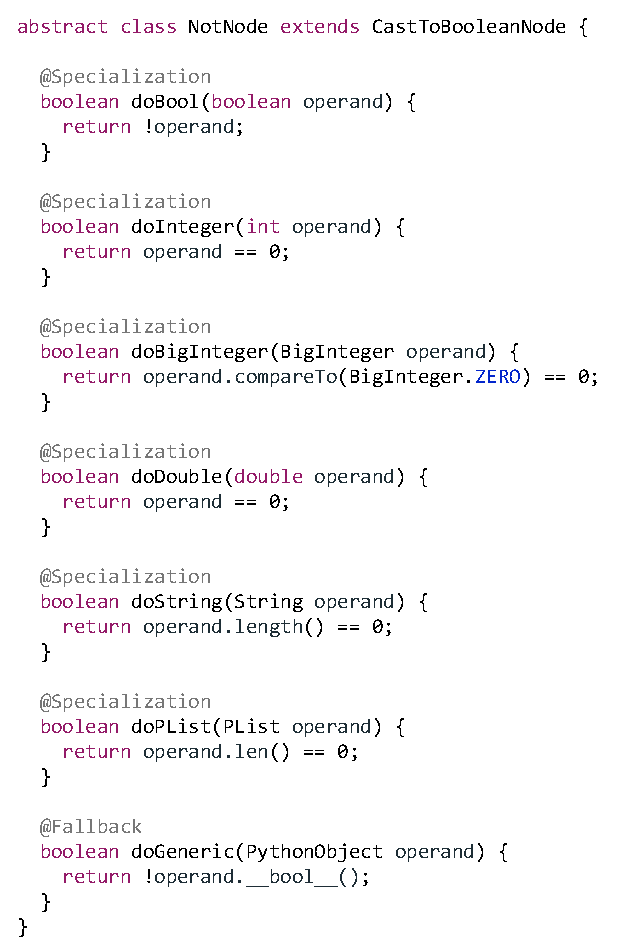
\includegraphics[scale=.8]{figures/ch3-not-node-code.pdf}
\caption{Implementation of \texttt{NotNode} in ZipPy}
\label{fig:not-node-code}
\end{figure}

\begin{figure}[t]
\centering
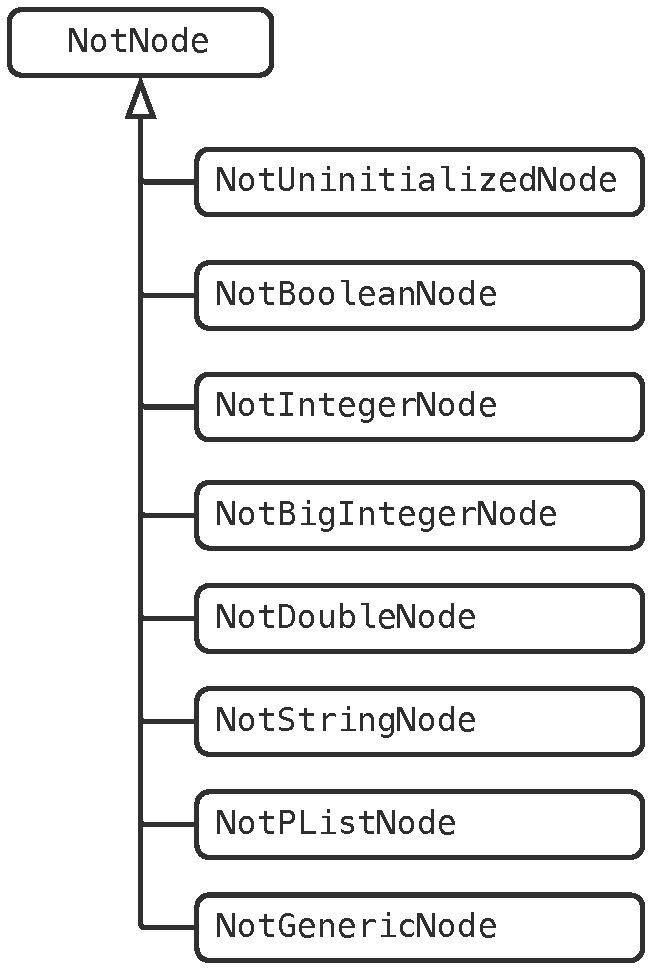
\includegraphics[scale=.5]{figures/ch3-not-node-derivatives.pdf}
\caption{Derivatives of \texttt{NotNode} in ZipPy}
\label{fig:not-node-derivatives}
\end{figure}

Truffle provides a Java annotation based source code generation engine.
Hosted VM implementers can use this engine to automatically generate type specialized derivatives for their AST interpreters.
Derivative generation is an essential but tedious part of applying type specializations.
This code generation process requires little boilerplate code from the hosted VM implementers and helps them to focus on the core logic of their interpreter.

\texttt{not} is a unary arithmetic operation in Python.
The operation evaluates the given expression to a boolean value and returns the inversion of that value.
Similar to other arithmetic operations, ZipPy implements \texttt{not} as a single AST node.
Figure~\ref{fig:not-node-code} illustrates the implementation of the \texttt{NotNode} in ZipPy using Truffle's DSL.
Note that each method annotated using \texttt{@Specialization} represents a type specialized derivative of the \texttt{NotNode}.
For instance, the method \texttt{doInteger} and \texttt{doDouble} implement the \texttt{not} operation for integers and floating point numbers.
We will explain in~\ref{sec:numeric-types} about the reason why we specialize against Java primitive types instead of boxed representations of numeric types in Python.
\texttt{@Fallback} denotes the generic version of the \texttt{not} operand.

Truffle's code generation engine produces the actual implementation of the derivative nodes.
Figure~\ref{fig:not-node-derivatives} shows the derivative classes produced by Truffle.
It generates a class for each method annotated with \texttt{@Specialization} in Figure~\ref{fig:not-node-code}.
The derivative nodes perform node rewriting based type specialization at runtime.
As shown in Figure~\ref{fig:python-on-truffle}, a \texttt{NotNode} starts with the uninitialized version.
At runtime, the node rewrites itself to a derivative that matches the type of the incoming operand.
The rewrite follows the order of the classes shown in Figure~\ref{fig:not-node-derivatives} from the top to the bottom.
If no matching derivative is found, the node rewrites to \texttt{NodeGenericNode}, which perform the generic routine for the \texttt{not} operation.

\subsection{Numeric Types}
\label{sec:numeric-types}

\subsection{Comnposite Data Types}

\chapter{Generator Peeling}
\label{chp:ch4-peeling}

Generators offer an elegant way to express iterators.
However, performance has always been their Achilles heel and has prevented widespread adoption.
We present techniques to efficiently implement and optimize generators.

We have implemented our optimizations in ZipPy, a modern, light-weight AST interpreter based Python 3 implementation targeting the Java virtual machine.
Our implementation builds on a framework that optimizes AST interpreters using just-in-time compilation.
In such a system, it is crucial that AST optimizations do not prevent subsequent optimizations.
Our system was carefully designed to avoid this problem.
We report an average speedup of \peelingSpeedup{}$\times$ for generator-bound programs.
As a result, using generators no longer has downsides and programmers are free to enjoy their upsides.

\section{Motivation}

Many programming languages support generators, which allow a natural expression of iterators.
We surveyed the use of generators in real Python programs, and found that among the 50 most popular Python projects
listed on the Python Package Index (PyPI)~\cite{pypi} and GitHub~\cite{github}, 90\% of these programs use generators.

Generators provide programmers with special control-flow transfers that allows function executions to be suspended and resumed.
Even though these control-flow transfers require extra computation, the biggest performance bottleneck is caused by preserving the state of a function between a suspend and a resume.
This bottleneck is due to the use of \emph{cactus} stacks required for state preservation.
Popular language implementations, such as CPython~\cite{python}, and CRuby~\cite{ruby}, allocate frames on the heap.
Heap allocation eliminates the need for cactus stacks, but is expensive on its own.
Furthermore, function calls in those languages are known to be expensive as well.

In this thesis, we examine the challenges of improving generator performance for Python.
First, we show how to efficiently implement generators in abstract syntax tree (AST) interpreters,
which requires a fundamentally different design than existing implementations for bytecode interpreters.
We use our own full-fledged prototype implementation of Python 3, called ZipPy\footnote{Publicly available at \url{https://bitbucket.org/ssllab/zippy}},
which targets the Java virtual machine (JVM).
ZipPy uses the Truffle framework~\cite{Wurthinger+13} to optimize interpreted programs in stages, first collecting type feedback in the AST interpreter,
then just-in-time compiling an AST down to optimized machine code.
In particular, our implementation takes care not to prevent those subsequent optimizations.
Our efficient generator implementation optimizes control-transfers via suspend and resume.

Second, we describe an optimization for frequently used idiomatic patterns of generator usage in Python.
Using this optimization allows our system to allocate generator frames to the native machine stack, eliminating the need for heap allocation.
When combined, these two optimizations address both bottlenecks of using generators in popular programming languages, and finally give way to high performance generators.

\noindent{}Summing up, our contributions are:

\begin{itemize}
\item We present an efficient implementation of generators for AST based interpreters that is easy to implement and enables efficient optimization offered by just-in-time compilation.
\item We introduce \emph{generator peeling}, a new optimization that eliminates overheads incurred by generators.
\end{itemize}

\section{Generators in Python}

A generator is a more restricted variation of a coroutine~\cite{grune1977view,Moura2009}.
It encompasses two control abstractions: \emph{suspend} and \emph{resume}.
\emph{Suspend} is a generator exclusive operation, while only the caller of a generator can \emph{resume} it.
Suspending a generator always returns control to its immediate caller.
Unlike regular subroutine calls, which start executing at the beginning of the callee, calls to a \emph{suspended} generator resume
from the point where it most recently suspended itself.
Those two operations are asymmetric as opposed to the symmetric control \emph{transfer} in coroutines.

\subsubsection*{Generator Functions}

\begin{figure}
\centering
\subfigure[Simple generator]{
	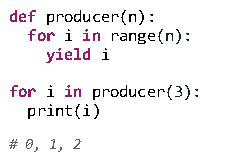
\includegraphics[scale=1.5]{figures/ch4-simple-generator-example-code}
	\label{fig:ch4-simple-generator-code}
}
\subfigure[Python iterator protocol]{
	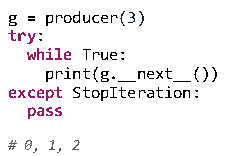
\includegraphics[scale=1.5]{figures/ch4-loop-on-generator-code}
	\label{fig:ch4-iterate-on-generator-code}
}
\caption{A simple generator function in Python}
\label{fig:ch4-generator-example}
\end{figure}

In Python, using the \texttt{yield} keyword in a function definition makes the function a generator function.
A call to a generator function returns a generator object without evaluating the body of the function.
The returned generator holds an execution state initialized using the arguments passed to the call.
Generators implement Python's iterator protocol, which includes a \texttt{\_\_next\_\_} method.
The \texttt{\_\_next\_\_} method starts or resumes the execution of a generator.
It is usually called implicitly, e.g., by a for loop that iterates on the generator (see Figure~\ref{fig:ch4-simple-generator-code}).
When the execution reaches a \texttt{return} statement or the end of the generator function, the generator raises a \texttt{StopIteration} exception.
The exception terminates generator execution and breaks out of the loop that iterates on the generator.
Figure~\ref{fig:ch4-iterate-on-generator-code} shows the desugared version of the for loop that iterates over the generator object \texttt{g} by explicitly calling \texttt{\_\_next\_\_}.

\subsubsection*{Generator Expressions}

\begin{figure}[h]
\centering
\subfigure[Generator expression]{
	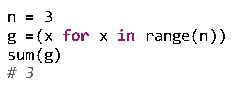
\includegraphics[scale=1.5]{figures/ch4-genexp-example-code}
	\label{fig:ch4-simple-genexp-code}
}
\subfigure[Desugared generator function]{
	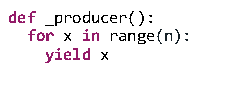
\includegraphics[scale=1.5]{figures/ch4-genexp-desugared-code}
	\label{fig:ch4-genexp-desugared-code}
}
\caption{A simple generator expression in Python}
\label{fig:ch4-genexp-example}
\end{figure}

Generator expressions offer compact definitions of simple generators in Python.
Generator expressions are as memory efficient as generator functions, since they both create generators that lazily produce one element at a time.
Programmers use these expressions in their immediate enclosing scopes.
Figure~\ref{fig:ch4-genexp-example} shows a simple generator expression and its equivalent, desugared generator function definition.
A generator expression defines an anonymous generator function, and directly returns a generator that uses the anonymous function definition.
The returned generator encapsulates its enclosing scope, if the generator expression references symbols in the enclosing scope (\texttt{n} in Figure~\ref{fig:ch4-genexp-example}).
The function \texttt{sum} subsequently consumes the generator by iterating on it in a loop and accumulating the values produced by the generator.

\subsubsection*{Idiomatic Uses of Generators}

\begin{figure}[h]
\centering
\subfigure[Generator loop]{
	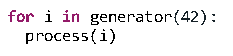
\includegraphics[scale=1.5]{figures/ch4-idiomatic-generator-loop-code}
	\label{fig:ch4-idiomatic-loop-code}
}
\subfigure[Implicit generator loop]{
	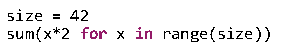
\includegraphics[scale=1.5]{figures/ch4-idiomatic-implicit-loop-code}
	\label{fig:ch4-idiomatic-implicit-code}
}
\caption{Idiomatic uses of generators}
\label{fig:ch4-idiomatic-patterns}
\end{figure}

The idiomatic way of using generators in Python is to write a \emph{generator loop}.
As shown in Figure~\ref{fig:ch4-idiomatic-loop-code}, a generator loop is a for loop that calls a generator function and consumes the returned generator object.
The common use pattern of a generator expression is to use it as a closure and pass it to a function that consumes it (see Figure~\ref{fig:ch4-idiomatic-implicit-code}).
The consumer functions, like \texttt{sum}, usually contain a loop that iterates on the generator.
Therefore, we refer to this pattern as an \emph{implicit generator loop}.
Explicit and implicit generator loops cover most of the generator usage in Python programs.
Our generator peeling optimization, which we explain in Section~\ref{sec:ch4-generaor-peeling}, targets these patterns.

\section{Generators Using an AST Interpreter}

Java, the host language of Truffle and ZipPy, does not offer native support for coroutines.
Our AST interpreter needs to model the semantics of generators.
However, the conventional way of implementing generators in a bytecode interpreter does not work in an AST setting.
In this section, we discuss the challenges of supporting generators in an AST interpreter, and present the solution we devised for ZipPy.

\subsection{AST Interpreters vs. Bytecode Interpreters}

\begin{figure}
\centering
\subfigure[Implementation of \texttt{WhileNode}]{
	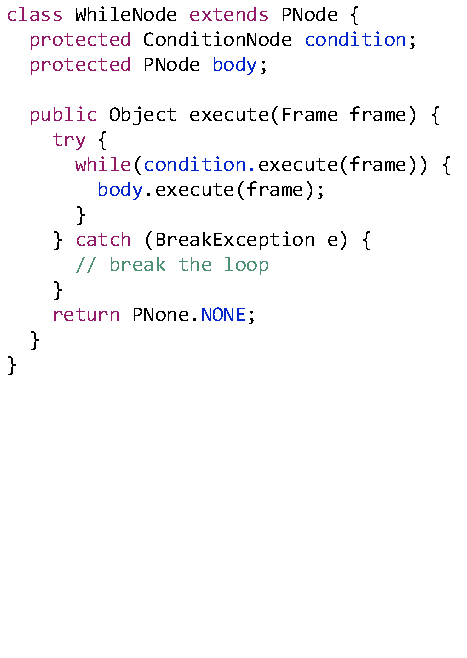
\includegraphics[scale=.9]{figures/ch4-while-node-code}
	\label{fig:ch4-while-node-code}
}
\subfigure[Implementation of \texttt{GenWhileNode}]{
	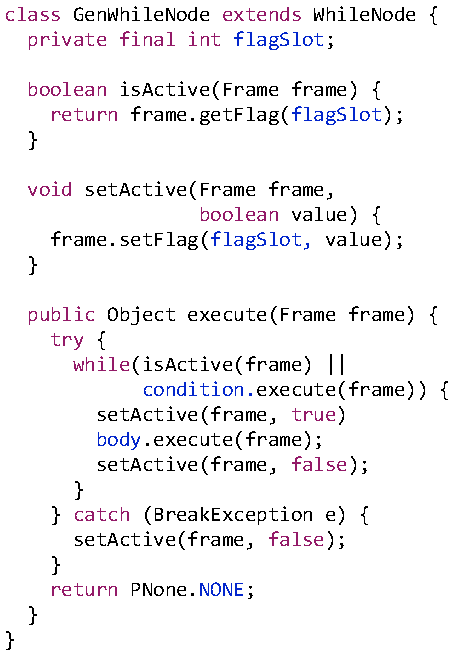
\includegraphics[scale=.9]{figures/ch4-gen-while-node-code}
	\label{fig:ch4-gen-while-node-code}
}
\caption{Two different \texttt{WhileNode} versions}
\label{fig:ch4-while-nodes}
\end{figure}

The de-facto Python implementation, CPython, uses bytecode interpretation.
It parses the Python program into a linearized bytecode representation and executes the program using a bytecode interpreter.
A bytecode interpreter is \emph{iterative}.
It contains an interpreter loop that fetches the next instruction in every iteration and performs its operation.
The bytecode index pointing to the next instruction is the only interpreter state that captures the current location of the program.
The interpreter only needs to store the program activation and the \emph{last} bytecode index when the generator suspends.
When resuming, a generator can simply load the program activation and the \emph{last} bytecode index before it continues with the next instruction.

An AST interpreter on the other hand is \emph{recursive}.
The program evaluation starts from the root node, then recursively descends to the leaves, and eventually returns to the root node.
In ZipPy, every AST node implements an \texttt{execute} method (see Figure~\ref{fig:ch4-while-nodes}).
Each \texttt{execute} method recursively calls the \texttt{execute} methods on its child nodes.
The recursive invocation builds a native call stack that captures the current location of the program.
The interpreter has to save the entire call stack when the generator suspends.
To resume the generator execution, it must rebuild the entire call stack to the exact point where it last suspended.

\subsection{Generator ASTs}
\label{sec:ch4-generator-ast}

ZipPy stores local variables in a heap-allocated frame object.
AST nodes access variables by reading from and writing to dedicated frame slots.
During just-in-time compilation, Truffle is able to map frame accesses to the machine stack and eliminate frame allocations.
However, a generator needs to store its execution state between a suspend and resume.
The frame object must therefore be kept on the heap which prevents Truffle's frame optimization.

In general, our AST interpreter implements control structures using Java's control structures.
We handle non-local returns, i.e., control flow from a deeply nested node to an outer node in the AST, using Java exceptions.
Figure~\ref{fig:ch4-genfunc-before} illustrates the AST of a Python generator function.
We model loops or if statements using dedicated \emph{control nodes}, e.g., a \texttt{WhileNode}.
The \texttt{BlockNode} groups a sequence of nodes that represents a basic block.
The \texttt{YieldNode} performs a non-local return by throwing a \texttt{YieldException}.
The exception bypasses the two parent \texttt{BlockNode}s, before the \texttt{FunctionRootNode} catches it.
The \texttt{FunctionRootNode} then returns execution to the caller.

\subsubsection*{Generator Control Nodes}

\begin{figure}
\centering
\subfigure[Before translation]{
	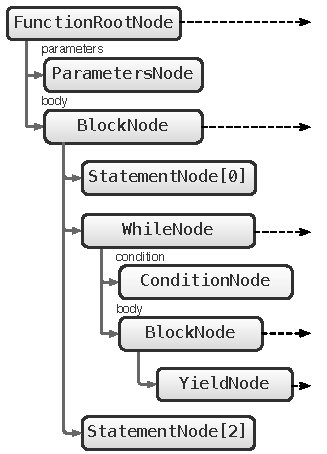
\includegraphics[scale=1.1]{figures/ch4-gen-function-orig}
	\label{fig:ch4-genfunc-before}
}
\subfigure[Translated]{
	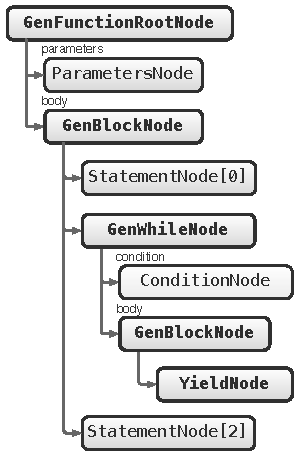
\includegraphics[scale=1.1]{figures/ch4-gen-function-translated}
	\label{fig:ch4-genfunc-translated}
}
\caption{Translation to generator AST}
\label{fig:ch4-genfunc-translation}
\end{figure}

Every control node in ZipPy has a local state stored in the local variables of its \texttt{execute} method.
The local state captures the current execution of the program, for instance, the current iterator of a for loop node or the current node index of a block node.
To support generators we decide to implement an alternative generator version for each control node.
These control nodes do not rely on local state, and keep all execution state in the frame.
However, it is overly conservative to use generator control nodes everywhere in a generator function.
We only need to use generator control nodes for the parent nodes of \texttt{YieldNode}s, since a yield operation only suspends the execution of these nodes.

Figure~\ref{fig:ch4-while-node-code} shows the implementation of a \texttt{WhileNode}.
Note that the loop condition result is a local state of the node stored in the call stack of its \texttt{execute} method.
When a \texttt{YieldException} is thrown somewhere in the loop body, it unwinds the call stack and discards the current loop condition result.
When the generator resumes, it will not be able to retrieve the previous loop condition result without re-evaluating the \texttt{condition} node.
The re-evaluation may have side effects and violate correct program behavior.
Therefore, this implementation only works for normal functions but not for generator functions.

Figure~\ref{fig:ch4-gen-while-node-code} shows the generator version of the \texttt{WhileNode}, the \texttt{GenWhileNode}.
It keeps an \emph{active} flag, a local helper variable, in the frame.
The \texttt{execute} method accesses the flag by calling the \texttt{isActive} or \texttt{setActive} method.
When a yield occurs in the loop body, the active flag remains true.
When resuming, it bypasses the condition evaluation and forwards execution directly to the loop body.

Note that it is incorrect to store the active flag as a field in the \texttt{GenWhileNode}.
Different invocations of the same generator function interpret the same AST, but should not share any state stored in the AST.
An alternative way to implement a \texttt{GenWhileNode} is to catch \texttt{YieldException}s in the \texttt{execute} method and set the active flag in the catch clause.
This implementation requires the \texttt{GenWhileNode} to re-throw the \texttt{YieldException} after catching it.
If we implement generator control nodes in this way, a yield operation will cause a chain of Java exception handling which is more expensive than the solution we chose.

Similar to the \texttt{GenWhileNode}, we implement a generator version for all the other control nodes in ZipPy.
Every generator control node has its own active flags stored in the frame.
The descriptions of the generator control nodes are as follows:

\begin{itemize}

\item \texttt{GenFunctionRootNode}:
Stores an active flag in the frame.
Only applies arguments when the flag is false.
Resets the flag and throws \texttt{StopIteration} exception upon termination of the generator.

\item \texttt{GenBlockNode}:
Stores the current node index in the frame.
Skips the executed nodes when the index is not zero.
Resets the index to zero upon exit.

\item \texttt{GenForNode}:
Stores the current iterator in the frame.
Resets the iterator to \texttt{null} upon exit.

\item \texttt{GenIfNode}:
Similar to \texttt{GenWhileNode}, uses an active flags to indicate which branch is active.

\item \texttt{GenWhileNode}:
See Figure~\ref{fig:ch4-gen-while-node-code}.

\item \texttt{GenBreakNode}:
Resets active flags of the parent control nodes up to the targeting loop node (the innermost enclosing loop), including the loop node.

\item \texttt{GenContinueNode}:
Resets active flags of the parent control nodes up to the targeting loop node, excluding the loop node.

\item \texttt{YieldNode}:
Must be a child of a \texttt{GenBlockNode}.
Evaluates and stores the yielding value in the frame before throwing the \texttt{YieldException}.
The root node then picks up the value and returns it to the caller.
The \texttt{YieldNode} also advances the statement index of its parent \texttt{BlockNode} to ensure that the generator resumes from the next statement.

\end{itemize}

\subsubsection*{Control Node Translation}
\label{sec:ch4-ast-of-gen-func}

ZipPy first parses Python functions into ASTs that use the \emph{normal} control nodes.
Generator functions require an additional translation phase that replaces the \emph{normal} control nodes with their \emph{generator} equivalents.
Figure~\ref{fig:ch4-genfunc-translation} illustrates this translation.
We only replace the control nodes that are parents of the \texttt{YieldNode}s, since these nodes fully capture the state required to suspend and resume execution.

The translated generator AST always keeps a snapshot of its execution in the frame.
When resuming, it is able to retrieve all the necessary information from the snapshot and rebuild the entire interpreter call stack to the exact point where it left off.

The flag accesses in the generator control nodes and the exception based control flow handling add performance overheads.
However, the underlying compiler is able to compile the entire generator AST into machine code.
It also optimizes control flow exceptions and converts them to direct jumps.
The jumps originate from where the exception is thrown and end at the location that catches it.
The AST approach, enforced by the underlying framework, does add complexity to the implementation of generators.
However, the performance gains offset this slight increase of the implementation effort.

\subsubsection*{Yield as an Expression}

\begin{figure}[h]
\centering
\subfigure[Yield expression]{
	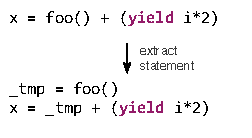
\includegraphics[scale=1.45]{figures/ch4-yield-expression-example}
	\label{fig:ch4-yield-expression-example}
}
\subfigure[Translated multiply]{
	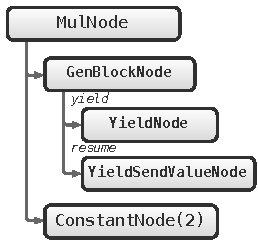
\includegraphics[scale=1.1]{figures/ch4-yield-expression-ast}
	\label{fig:ch4-yield-expression-ast}
}
\caption{Translation of a yield expression}
\label{fig:ch4-yield-expression}
\end{figure}

Python allows programmers to use yield in expressions.
A yield expression returns a value passed from the caller by calling the generator method \texttt{send}.
This enhancement allows the caller to pass a value back to the generator when it resumes, and brings generators closer to coroutines.
However, it requires generator ASTs to be able to resume to a specific expression.

Figure~\ref{fig:ch4-yield-expression-example} shows an example of yield expressions.
The assignment statement to variable \texttt{x} consumes the value returned by the yield expression.
Figure~\ref{fig:ch4-yield-expression-ast} shows the translated AST of the multiplication sub-expression.
Note that we translate the yield expression to a \texttt{GenBlockNode} containing a \texttt{YieldNode} and a \texttt{YieldSendValueNode}.
When the \texttt{YieldNode} suspends execution, it advances the active node index of the parent \texttt{GenBlockNode} to point to the next node.
This action ensures that the generator restarts execution from the \texttt{YieldSendValueNode}, which returns the value sent from the caller.

In a more complicated case, the statement consuming the yield expression could contain sub-expressions with a higher evaluation order.
In other words, the interpreter should evaluate these expressions before the yield expression.
Some of them could have side effects, i.e., the call to \texttt{foo} in Figure~\ref{fig:ch4-yield-expression-example}.
To avoid re-evaluation, we convert such expressions into separate statements and create variables to store the evaluated values.
When the generator resumes, it picks up the evaluated values from the variables without visiting the expression nodes again.

\section{Optimizing Generators with Peeling}
\label{sec:ch4-generaor-peeling}

Generator peeling is an AST level speculative optimization that targets the idiomatic generator loop pattern.
It transforms the high level generator calling semantics to lower level control structures and eliminates the overheads incurred by generators altogether.

\subsection{Peeling Generator Loops}

\begin{figure}[ht]
\centering
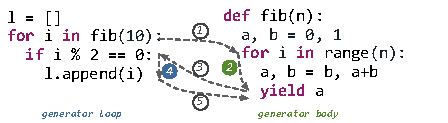
\includegraphics[scale=1.5]{figures/ch4-gen-exec-order}
\caption{Program execution order of a generator loop}
\label{fig:ch4-gen-exec-order}
\end{figure}

Figure~\ref{fig:ch4-gen-exec-order} shows a generator loop (left) that collects even numbers among the first ten Fibonacci numbers generated by \texttt{fib} (right) into the list \texttt{l}.
For each iteration in the loop, the program performs the following steps:

\begin{enumerate}
\item Call \texttt{\_\_next\_\_} on the generator and resume execution.

\item Perform another iteration in the for \texttt{range} loop to compute the next Fibonacci number.

\item Return the value of \texttt{a} to the caller and assign it to \texttt{i}.

\item Execute the body of the generator loop.

\item Return to the loop header and continue with the next iteration.
\end{enumerate}

Among those steps listed above, only step two and four perform the actual computation.
Steps one and three are generator specific resume and suspend steps.
They involve calling a function, resuming the generator AST to the previous state and returning the next value back to the caller.
Those generator specific steps add high overhead to the real work in the generator loop.

The most common and effective technique for optimizing function calls is to inline callees into callers.
However, traditional function inlining does not work for generators.
The desugared generator loop (similar to the one shown in Figure~\ref{fig:ch4-iterate-on-generator-code}) includes two calls: one to the generator function \texttt{fib} and another one to the \texttt{\_\_next\_\_} method.
The call to \texttt{fib} simply returns a generator object during loop setup, and is not performance critical.
Inlining the call to \texttt{\_\_next\_\_} requires special handling of \emph{yield}s rather than treating them as simple returns.
An ideal solution should handle both calls at the same time, while still preserving semantics.

Observe that the generator loop always calls \texttt{\_\_next\_\_} on the generator unless it terminates.
If the generator loop body was empty, we can replace the loop with the generator body of \texttt{fib} and still preserve semantics.
Furthermore, assuming the above mentioned replacement is in-place, for the non-empty loop body case, we can replace each yield statement with the generator loop body.
Figure~\ref{fig:ch4-peeling-trans} illustrates this transformation.
The solid arrow depicts the generator loop replacement that ``inlines'' the generator body.
The dashed arrow shows the yield replacement that combines the generator code and the caller code.

Figure~\ref{fig:ch4-fib-peeled} shows the pseudo-code of the transformed program.
We combine the generator body and the loop body in the same context.
The original call to the generator function \texttt{fib} translates to the assignment to \texttt{n} which sets up the initial state of the following generator body.
The generator body replaces the original generator loop.
We simplify the yield statement to a single assignment.
The assignment transfers the value of \texttt{a} from the generator body to the following loop body.
The loop body in turn consumes the ``yielded'' value of \texttt{i}.

\begin{figure}[!t]
\centering
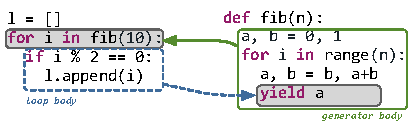
\includegraphics[scale=1.5]{figures/ch4-peeling-generator-call}
\caption{Peeling transformation}
\label{fig:ch4-peeling-trans}
\end{figure}

\begin{figure}[!t]
\centering
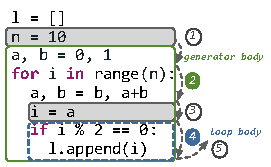
\includegraphics[scale=1.5]{figures/ch4-fib-peeled}
\caption{Transformed generator loop}
\label{fig:ch4-fib-peeled}
\end{figure}

The transformation peels off the generator loop, and removes both calls, to \texttt{fib} and \texttt{\_\_next\_\_}.
The optimized program does not create a generator object.
It eliminates the step one and simplifies the step three shown in Figure~\ref{fig:ch4-gen-exec-order}.
These two steps do not contribute to the real computation.
The numbers on the right of Figure~\ref{fig:ch4-fib-peeled} denote the corresponding execution steps of the original generator loop shown in Figure~\ref{fig:ch4-gen-exec-order}.
The two assignments preceding the transformed generator body and the loop body (grayed in Figure~\ref{fig:ch4-fib-peeled}) preserve the correct data flow into and out of the generator code.

We simplified the pseudo code shown in Figure~\ref{fig:ch4-fib-peeled} for clarity.
Our transformation is not limited to the case where the call to the generator function happens at the beginning of the consuming loop.
If the creation of the generator object happens before the loop, we apply the same transformation that combines the generator body with the loop body.
We explain the actual AST transformation in more detail in Section~\ref{sec:ch4-ast-transformation}.

\subsection{Peeling AST Transformations}
\label{sec:ch4-ast-transformation}

\begin{figure*}
\centering
\subfigure[AST transformation]{
	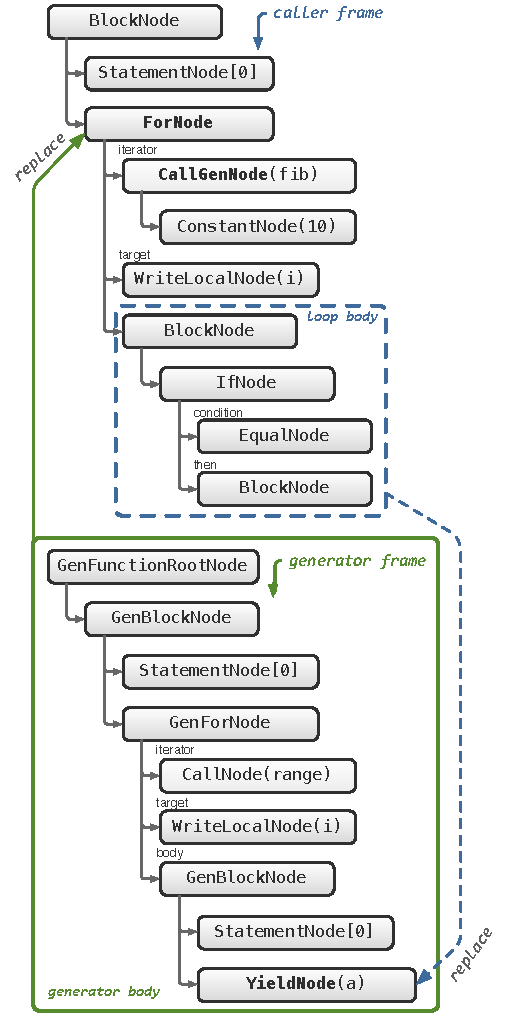
\includegraphics[scale=.82]{figures/ch4-ast-before-peeling}
	\label{fig:ch4-ast-before-peeling}
}
\subfigure[Transformed generator loop AST]{
	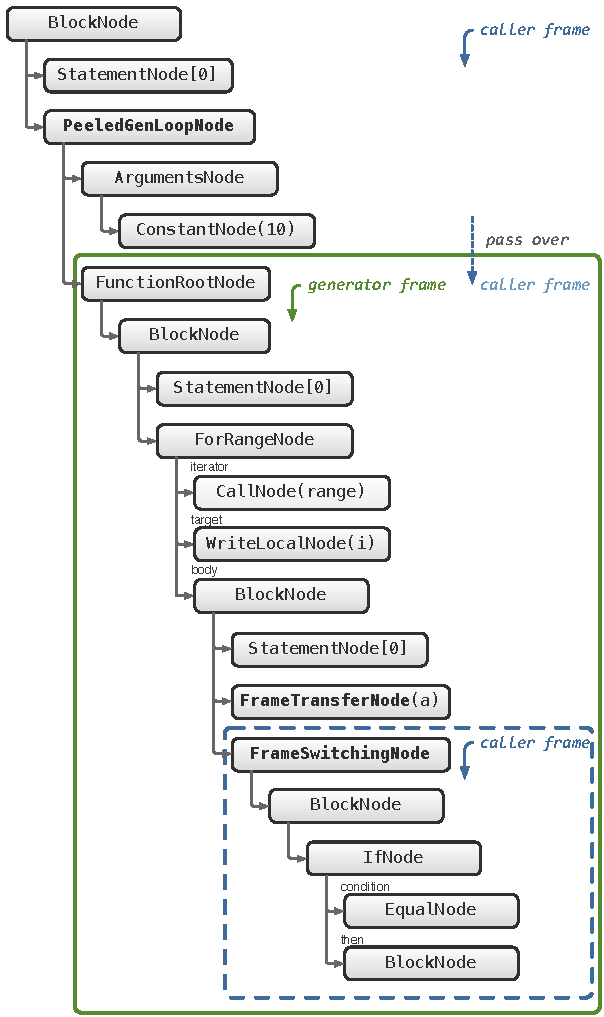
\includegraphics[scale=.82]{figures/ch4-peeled-ast}
	\label{fig:ch4-peeled-ast}
}
\caption{Peeling AST transformation}
\label{fig:ch4-ast-transformation}
\end{figure*}

Figure~\ref{fig:ch4-ast-before-peeling} shows the AST transformation of our Fibonacci example.
The upper half of the figure shows the AST of the generator loop.
The AST contains a \texttt{CallGenNode} that calls the generator function \texttt{fib}, and returns a generator object to its parent node.
The parent \texttt{ForNode} representing the for loop then iterates over the generator.
The lower half of the figure shows the AST of the generator function \texttt{fib}.
Note that the generator body AST uses generator control nodes and includes the \texttt{YieldNode} that returns the next Fibonacci number to the caller.

The figure also illustrates the two-step peeling AST transformation.
First we replace the \texttt{ForNode} that iterates over the generator with the AST of the generator body.
Second, we clone the AST of the loop body and use it to replace the \texttt{YieldNode} in the generator body.
Figure~\ref{fig:ch4-peeled-ast} shows the result of the transformation.
We use a \texttt{PeeledGenLoopNode} to guard the transformed generator body.
The \texttt{PeeledGenLoopNode} receives the arguments from the \texttt{ArgumentsNode} and passes them the transformed generator body.
The \texttt{FrameTransferNode} transfers the Fibonacci number stored in the variable \texttt{a} to the following loop body (equivalent to step three in Figure~\ref{fig:ch4-fib-peeled}).
The transformed loop body in turn consumes the ``yielded'' number.

ZipPy implements a number of different versions of \texttt{PeeledGenLoopNode} to handle different loop setups.
For instance, a generator loop could consume an incoming generator object without calling the generator function at the beginning of the loop.
The transformed \texttt{PeeledGenLoopNode} in this case guards against the actual call target wrapped by the incoming generator object and receives the arguments from the generator object.

\subsection{Polymorphism and Deoptimization}
\label{sec:ch4-polymorphic-and-deopt}

ZipPy handles polymorphic operations by forming a chain of specialized nodes with each node implementing a more efficient version of the operation for a particular operand type.
The interpreter then dispatches execution to the desired node depending on the actual type of the operand.
Like other operations in Python, the type of the iterator coming into a loop can change at runtime.
A loop that iterates over multiple types of iterators is a polymorphic loop.

\begin{figure}
\centering
\subfigure[Monomorphic]{
	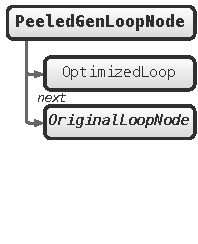
\includegraphics[scale=1.15]{figures/ch4-ast-peeled-mono}
	\label{fig:ch4-ast-peeled-mono}
}
\subfigure[Polymorphic]{
	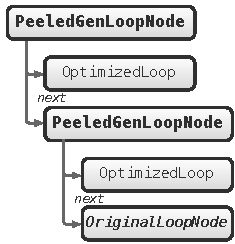
\includegraphics[scale=1.15]{figures/ch4-ast-peeled-poly}
	\label{fig:ch4-ast-peeled-poly}
}
\subfigure[Deoptimized]{
	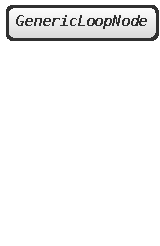
\includegraphics[scale=1.15]{figures/ch4-ast-peeled-deopt}
	\label{fig:ch4-ast-peeled-deopt}
}
\caption{Handling of polymorphic generator loop}
\label{fig:ch4-peeling-polymorphic}
\end{figure}

Generator peeling is a loop specialization technique that targets generators, a particular kind of iterators.
ZipPy handles polymorphic loops by forming a chain of specialized loop nodes including \texttt{PeeledGenLoopNode}s.
A \texttt{PeeledGenLoopNode} checks the actual call target of the incoming iterator before it executes the optimized loop.
As shown in Figure~\ref{fig:ch4-peeling-polymorphic}, if the target changes, then the execution falls through to the original loop node.
ZipPy is able to apply an additional level of the generator peeling transformation for the new iterator type if it happens to be a generator as well.

However, forming a polymorphic chain that is too deep could lead to code explosion.
If the depth of the chain goes beyond a pre-defined threshold, ZipPy stops optimizing the loop and replaces the entire chain with a generic loop node.
The generic loop node is capable of handling all types of incoming iterators but with limited performance benefit.

\subsection{Frames and Control Flow Handling}
\label{sec:ch4-frame-and-control}

The AST of the optimized generator loop combines nodes from two different functions and therefore accesses two different frame objects.
Programmers can use non-local control flows such as \texttt{break}s or \texttt{continue}s in a generator loop body.
We explain how to handle frames and such control flows in the rest of this section.

\subsubsection*{Frame Switching}

% two frames in the fig
The transformed AST illustrated in Figure~\ref{fig:ch4-peeled-ast} accesses two frames: the caller frame and the generator frame.
Figure~\ref{fig:ch4-two-frames} shows the layouts of the two frames.
The nodes belonging to the caller function read from and write to the caller frame to access its local variables.
The generator body nodes do so through the generator frame.
The \texttt{PeeledGenLoopNode} allocates the generator frame and passes it to the dominated generator body.
To enable caller frame access in the deeply nested loop body, the node also passes over the caller frame.
Therefore, in the sub-tree dominated by the \texttt{PeeledGenLoopNode}, both frames are accessible.

\begin{figure}[!ht]
\centering
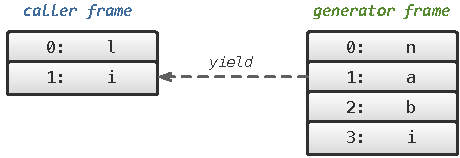
\includegraphics[scale=1.2]{figures/ch4-two-frames}
\caption{The caller and generator frame objects of the Fibonacci example}
\label{fig:ch4-two-frames}
\end{figure}

% passing caller over and switches between two frames
Although keeping both frames alive and accessible, the interpreter picks one frame object as the current frame and retains the other one as the background frame.
It passes the current frame to every \texttt{execute} method of the AST nodes as an argument for faster access.
The current frame stores a reference to the background frame.
The accesses to the background frame require one more level of indirection.

In the generator body shown in Figure~\ref{fig:ch4-peeled-ast}, the interpreter sets the generator frame as the current frame.
The \texttt{FrameTransferNode} propagates the values of \texttt{a} in the generator frame to \texttt{i} in the caller frame.
This value propagation corresponds to step 3 in Figure~\ref{fig:ch4-gen-exec-order} and Figure~\ref{fig:ch4-fib-peeled}.
The following \texttt{FrameSwitchingNode} swaps the positions of the two frames and passes the caller frame as the current frame to the dominated loop body.

% truffle remove frame allocation.
Truffle's underlying JIT compiler optimizes frame accesses.
It eliminates frame allocations as long as references to the frame object are not stored on the heap.
A generator stores its execution state by keeping a frame object reference on the heap.
Therefore, the generator AST introduced in Section~\ref{sec:ch4-generator-ast} prevents this frame optimization.
After generator peeling, however, the program does not create and iterate over generators.
It is not necessary to adopt generator control nodes in the ``inlined'' generator body and store frame object references on the heap.
As a result, the compiler can successfully optimize frame accesses in the transformed generator loop regardless of the number of frames.

For generator functions containing multiple yields, we apply the same transformation to each \texttt{YieldNode}.
The resulting AST contains more than one loop body, hence multiple \texttt{FrameSwitchingNode}s.
We rely on the control-flow optimizations of the underlying compiler to minimize the cost of this replication.

Merging both frames could also guarantee correct frame accesses in the transformed AST.
However, this approach is more complicated.
Merging frames combines the allocations of both frames, which requires redirecting all frame accesses to the combined frame.
Upon deoptimization, we need to undo the merge and redirect all frame accesses back to their separate frames.
This process become more complex for the nested generator loop scenario which we explain more in Section~\ref{sec:ch4-multilevel-peeling}.
Since the underlying compiler is able to optimize multiple frame objects, merging frames does not produce faster code.

\subsubsection*{Breaks and Continues}

\begin{figure}
\centering
\subfigure[Break handling]{
	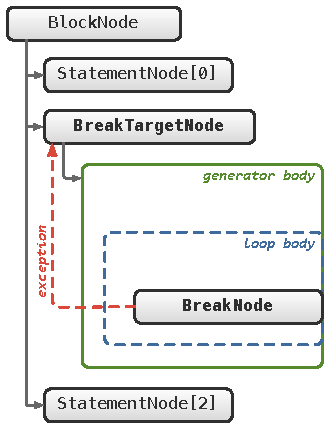
\includegraphics[scale=1.1]{figures/ch4-break-handling}
	\label{fig:ch4-break-handling}
}
\subfigure[Continue handling]{
	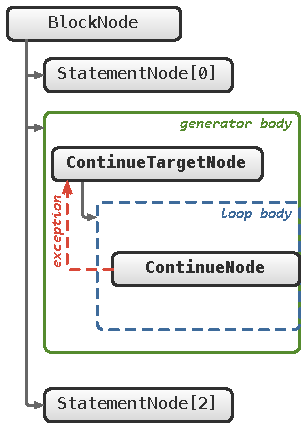
\includegraphics[scale=1.1]{figures/ch4-continue-handling}
	\label{fig:ch4-continue-handling}
}
\caption{Complex control flow handling}
\label{fig:ch4-break-and-continue}
\end{figure}

ZipPy implements break and continue statements using Java exceptions.
A \texttt{BreakNode} throws a break exception, and then a parent node catches the exception.
The control flow exception skips all the nodes between the throwing node and the catching node.
The location of the catch clause determines what the exception can skip.
Figure~\ref{fig:ch4-gen-while-node-code} shows the catch clause in a \texttt{GenWhileNode}.
The node catches the break exception after the while loop, hence the exception breaks the loop.
Similarly, a continue exception caught in the loop body quits the current iteration and continues with the next iteration.
There are no labeled break or continue statements in Python.
Thus, a control flow exception does not go beyond its enclosing loop.
Furthermore, we can extract the exception catch clauses to dedicated nodes to construct more complicated control structures.

A generator loop body may contain break or continue statements that target the generator loop.
Generator peeling replaces the generator loop and embeds the loop body inside the generator body.
To properly handle breaks in the loop body, we interpose a \texttt{BreakTargetNode} between the caller and the generator body as shown in Figure~\ref{fig:ch4-break-handling}.
The nested \texttt{BreakNode} throws a dedicated break exception to skip the generator body, before it reaches the \texttt{BreakTargetNode}.
After catching the exception, the \texttt{BreakTargetNode} returns to its parent and skips the rest of the generator loop.
We handle continues by interposing a \texttt{ContinueTargetNode} between the loop body and the generator body (see Figure~\ref{fig:ch4-continue-handling}).
A continue exception skips the rest of the nodes in the loop body and returns execution to the generator body.
This control flow is equivalent to what a continue does in the original generator loop, that is resuming the generator execution from the statement after the last yield.

The above mentioned interposition is only necessary when the optimized loop body contains break or continue statements.
As we explained in Section~\ref{sec:ch4-ast-of-gen-func}, the underlying compiler optimizes control-flow exceptions into direct jumps.
Therefore, the exception-based control handling has no negative impact on peak performance.

\subsection{Implicit Generator Loops}

\begin{figure}[th]
\centering
\subfigure[Original]{
	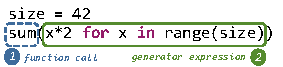
\includegraphics[scale=1.5]{figures/ch4-implicit-orig}
	\label{fig:ch4-implicit-orig}
}

\subfigure[Inlined]{
	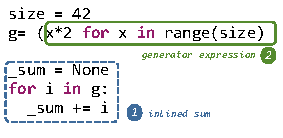
\includegraphics[scale=1.5]{figures/ch4-implicit-inlined}
	\label{fig:ch4-implicit-inlined}
}

\subfigure[Desugared]{
	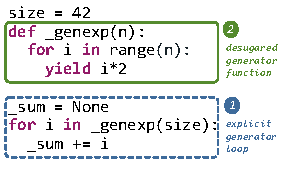
\includegraphics[scale=1.5]{figures/ch4-implicit-desugared}
	\label{fig:ch4-implicit-desugared}
}
\caption{Implicit generator loop transformation}
\label{fig:ch4-implicit-gen-loop}
\end{figure}

An implicit generator loop consists of a generator expression that produces a generator, and a function call that consumes the generator.
ZipPy applies additional transformation on implicit generator loops to enable further optimizations such as generator peeling.

Figure~\ref{fig:ch4-implicit-gen-loop} illustrates this two-step process.
First, we inline the function \texttt{sum} to expose the loop that consumes the generator (see Figure~\ref{fig:ch4-implicit-inlined}).
The inlining step triggers an escape analysis of all the generator expressions in the current scope.
If our analysis finds a generator expression such that the generator it produces does not escape the current scope and
a generator loop that consumes the produced generator exists, ZipPy desugars the expression to a generator function (see Figure~\ref{fig:ch4-implicit-desugared}).
Note that the desugared generator function redirects the references to the enclosing scope to the argument accesses in the local scope.
This redirection eliminates non-local variables in the generator expression and allows the compiler optimization for the enclosing frame.
The desugaring also replaces the generator reference in the inlined loop to a function call.
The transformation exposes the explicit generator loop that we can optimize using generator peeling.

One obstacle when optimizing an implicit generator loop is that the function consuming the generator can be a Python built-in function.
Programmers can use any built-in function that accepts iterable arguments in an implicit generator loop.
Table~\ref{tab:ch4-builtins} lists all the Python 3 built-in functions that accept iterables and divides them into three different categories:

\begin{table}[!ht]
  \begin{center}
    \begin{tabular}{ c c c }
      \toprule
      1. Implement in                & 2. Synthesize to loop & 3. No loop \\
      Python                         &                       & \\
      \midrule
      \texttt{all}, \texttt{any}     & \texttt{bytes}        & \texttt{iter} \\
      \texttt{bytearray}             & \texttt{dict}         & \texttt{next} \\
      \texttt{enumerate}             & \texttt{frozenset}    &               \\
      \texttt{filter}, \texttt{list} & \texttt{set}          &               \\
      \texttt{map}, \texttt{max}     & \texttt{tuple}        &               \\
      \texttt{min}, \texttt{sorted}  &                       &               \\
      \texttt{sum}, \texttt{zip}     &                       &               \\
      \bottomrule
    \end{tabular}
    % \nocaptionrule{}
    \caption{Python Built-in functions that accept iterables}
    \label{tab:ch4-builtins}
  \end{center}
\end{table}

\begin{enumerate}

\item \textbf{Implement in Python}:
Convenience functions that one can write in pure Python.
ZipPy implements these functions using Python code.
They share the same inlining approach with user defined functions.

\item \textbf{Synthesize to loop}:
Constructors of immutable data types in Python.
Cannot be written in pure Python without exposing internal data representations of the language runtime.
The current solution is to speculatively intrinsify the built-in call by replacing the call node with a synthesized AST.
The synthesized AST contains the generator loop and constructs the desired data type.
The intrinsified call site exposes the generator loop and enjoys the same peeling optimization.

\item \textbf{No loop}:
Contains no loop.
We exclude them from the optimization.

\end{enumerate}

\subsection{Multi-level Generator Peeling}
\label{sec:ch4-multilevel-peeling}

ZipPy relies on the tiered execution model of the underlying framework.
It starts executing a Python program in interpretation mode.
The interpreter collects runtime information and inlines function calls that are hot.
We apply function inlining using an inlining budget.
This budget helps to prevent code explosions caused by inlining too many calls or too big a callee.
We perform generator peeling when a generator function call becomes hot, and possibly bail out if the transformation did not succeed.
Generator peeling shares its budget with function inlining.
If a generator peeling transformation is going to overrun the inlining budget, ZipPy aborts the transformation.
After exhausting all possible inlining and peeling opportunities, Truffle compiles the entire AST into machine code.
All subsequent calls to the compiled function execute at peak performance.

\begin{figure}
\centering
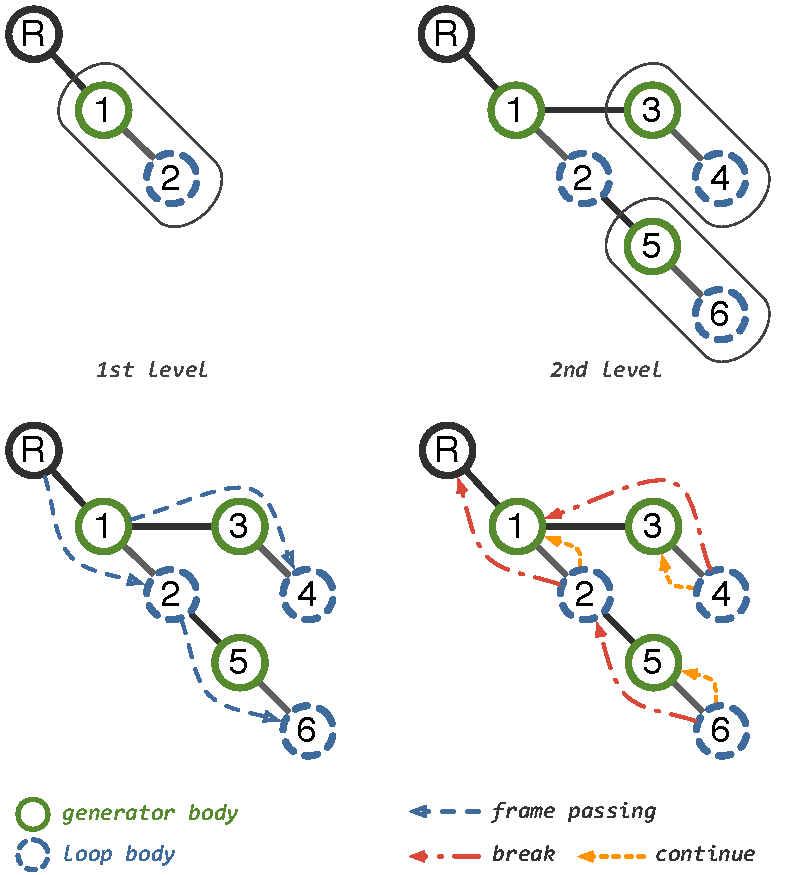
\includegraphics[scale=.9]{figures/ch4-multilevel-peeling}
\caption{Multi-level generator peeling}
\label{fig:ch4-multilevel-peeling}
\end{figure}

An optimized generator loop might include another generator loop.
We call these cases nested generator loops.
Python programs can contain arbitrary levels of nested generator loops.
Our optimization is capable of handling multiple levels of nested generator loops by iteratively peeling one loop layer at a time.
It requires minimal modifications to our existing algorithms to handle this scenario.

Figure~\ref{fig:ch4-multilevel-peeling} shows the AST of three nested generator loops after peeling transformations.
In a simple case, an optimized generator loop consists of two parts: the inlined generator body and the embedded loop body.
To illustrate the relationships between these two program regions, we simplify the structure of the AST by using one node for each program region.
A numbered solid circle denotes a generator body, and a numbered dashed circle denotes a loop body.
An ``inlined'' generator body node is always associated with a loop body node as its immediate child.
As shown in Figure~\ref{fig:ch4-multilevel-peeling}, the first level peeling results in node one being the generator body and node two being the loop body.
The second level peeling includes two optimized generator loops with nodes three and four extended from the generator body and nodes five and six extended from the loop body.
Note that at any level in the tree, a next level peeling can either extend from the generator body or the loop body of the current level.
More complicated cases recursively repeat the same tree structure as shown in Figure~\ref{fig:ch4-multilevel-peeling}.
Therefore, a working solution for the shown tree structure automatically extends to more complicated cases.

% rules in the tree
The tree shown in the figure adheres to the following rules:
Since it is a tree, every node only has one parent except the root node.
Every solid node has an associated dashed node as its child but possibly not the only child.
Every dashed node has an associated solid node as its only parent.
Every dashed node must have one and only one grandparent.

The arrows in Figure~\ref{fig:ch4-multilevel-peeling} depict the desired frame and control-flow handling.
Every dashed node receives two frames: one from its parent and another one from its grandparent.
Since every dashed node has a unique parent and a unique grandparent, there it no ambiguity on which two frames it receives.
A \texttt{continue} returns from a dashed node to its associated solid node.
Since the associated solid node is its only parent, no node can intercept this control-flow.
Our existing algorithms therefore automatically cover frame handling and continue statements for nested generator loops.

Break statements are more complicated.
A \texttt{break} returns from a dashed node to its grandparent.
However, its solid parent node may be the break target of another node and intercept the break exception.
For instance, node one in the figure might catch the break exception thrown in node two or node four.
This ambiguity may cause an incorrect break from node two.
To resolve this issue, we need to label the overlapping break exceptions to filter out undesired ones.
Since it is rare to have two nested generator loops that both use breaks, we consider this scenario as a corner case.

In summary, our peeling transformation is able to handle arbitrary levels of nested generator loops.

% ... and so on

% These commands fix an odd problem in which the bibliography line
% of the Table of Contents shows the wrong page number.
\clearpage
\phantomsection

% "References should be formatted in style most common in discipline",
% abbrv is only a suggestion.
\bibliographystyle{abbrv}
\bibliography{thesis}

% The Thesis Manual says not to include appendix figures and tables in
% the List of Figures and Tables, respectively, so these commands from
% the caption package turn it off from this point onwards. If needed,
% it can be re-enabled later (using list=yes argument).
\captionsetup[figure]{list=no}
\captionsetup[table]{list=no}

% If you have an appendix, it should come after the references.
\include{appendix}

\end{document}
